\documentclass[prb,showpacs,amsmath,amssymb,superscriptaddress,twocolumn,floatfix]{revtex4-1}

\usepackage{graphicx}
\usepackage{color}
\usepackage{amsmath}
\usepackage{hyperref}
\hypersetup{breaklinks=true}


\def\unit#1{\ \mathrm{#1}}
\def\Rea{\mbox{Re }}
\def\Ima{\mbox{Im }}
\def\ve{\varepsilon}
\def\veeff{\ve_{\mathrm{eff}}}
\def\atan{\mbox{atan }}
\def\asin{\mbox{asin }}
\def\Tr{\mbox{Tr }}

%%% fte-list
% fig-01, fig-02, fig-03, fig-04
% tab-01
% eq-01, eq-02, eq-03, eq-04, eq-05, eq-06, eq-07, eq-08, eq-09, eq-10
% eq-11, eq-12, eq-13, eq-14, eq-15, eq-16, eq-17, eq-18, eq-19, eq-20
% eq-21, eq-22, eq-23, eq-24, eq-25, eq-26, eq-27, eq-28, eq-29, eq-30
% eq-31, eq-32, eq-33, eq-34, eq-35

\begin{document}

\title{Non-Relativistic Anisotropic Magnetoresistance}

\author{P. Ritzinger}
%\affiliation{Institute of Physics, ASCR, $v.~v.~i.$, 
%	Cukrovarnick\'a 10, CZ-16253 Praha 6, Czech Republic}

\author{O. Sedl\'a\v cek}
\author{J. \v Zelezn\'y}

\author{K. V\'yborn\'y}
\affiliation{Institute of Physics, ASCR, $v.~v.~i.$, 
Cukrovarnick\'a 10, CZ-16253 Praha 6, Czech Republic}


\date{Jun04, 2025}

\begin{abstract}
Anisotropic magnetoresistance (AMR) is a manifestation of
magnetic-order-induced symmetry lowering of conductivity tensor. While the AMR in simple ferromagnets is usually considered to be a relativistic effect (it relies on spin-orbit interaction), we show that symmetry lowering, similar in spirit, can also happen in a non-relativistic limit. Using tight-binding models and Boltzmann transport theory, we investigate systems with multiple magnetic sublattices, including both collinear and non-collinear antiferromagnets, as well as ferrimagnetic configurations. We show that AMR and related anisotropies can emerge purely from magnetic order, without spin–orbit interaction, and may reach appreciable magnitudes. The findings are supported by case studies on toy-model lattices and real materials such as MnN, Mn$_3$Sn, and EuTe$_2$, and are further interpreted through symmetry analysis based on Neumann’s principle.
\end{abstract}

%\pacs{75.47.-m}
% 75.47.-m  Magnetotransport phenomena; materials for magnetotransport
%           (for spintronics, see 85.75.-d; see also 72.15.Gd, 73.50.Jt,
%           73.43.Qt, and 72.25.-b in transport phenomena)

\maketitle


\section{Introduction}

Anisotropic magnetoresistance (AMR), first observed by William Thomson in 1857~\cite{Thomson:1857}, describes the dependence of resistivity in ferromagnetic materials such as cobalt and nickel on the direction of magnetization. Since then, AMR has remained an active subject of research~\cite{Ritzinger:2023}. In its prototypical form, AMR is observed in polycrystalline ferromagnets (FMs), where it manifests as a two-fold (180$^\circ$-periodic) angular dependence of resistivity $\rho$ on the angle $\varphi$ between the current and the magnetization direction~\cite{Alagoz:2015}:
%
\begin{equation}
	\frac{\Delta \rho}{\rho} \propto \cos 2\varphi
	\label{eq_ncollAMR}
\end{equation}
%
This implies that, for example, if the magnetization in an otherwise isotropic medium ($\sigma_{xx} = \sigma_{yy}$ above the magnetic ordering temperature) is oriented along the $x$-direction, the conductivity tensor $\boldsymbol{\sigma} = \boldsymbol{\rho}^{-1}$ becomes anisotropic with $\sigma_{xx} \neq \sigma_{yy}$.

The conventional understanding of AMR~\cite{Vitayaya:2024}, in line with Eq.~\ref{eq_ncollAMR}, relies on spin-orbit coupling (SOC), which couples the spin of electrons to the crystal lattice. However, this description is not exhaustive. In this work, we demonstrate that similar symmetry-lowering effects in the conductivity tensor can also arise in the absence of SOC, provided the magnetic order involves multiple magnetic sublattices (MSLs), including both collinear and non-collinear magnetically ordered systems.

\subsection{Definition of AMR}

More generally, AMR can be defined as the change in symmetry of the conductivity tensor $\sigma_{ij}$ due to magnetic ordering. This includes the standard formulation in Eq.~\ref{eq_ncollAMR}, but excludes anisotropy of orbital (induced merely by Lorentz force) magnetoresistance in non-magnetic systems, or surface states in topological insulators~\cite{Ritzinger:2023}. Historically, AMR has also appeared under various names in the literature—such as spontaneous magnetoresistance anisotropy (SMA)—though these are not always consistently defined throughout literature~\cite{Ritzinger:2023}. The above definition offers a general framework encompassing these different terminologies.

We distinguish two ways of how AMR is commonly {\color{red}understood/measured --- not sure, what's better to say}:

\begin{enumerate}
	\item \textit{Rotation of magnetic order:} This is the most widely used experimental approach. In single-MSL ferromagnets (such as iron, cobalt, nickel and their alloys), AMR can be easily measured while the magnetic order is rotated using an applied magnetic field. This approach is applied also in other systems with collinear magnetic order, such as antiferromagnets (AFMs) like MnTe~\cite{Kriegner:2017, Gonzalez-Betancourt:2024} and CuMnAs~\cite{Volny:2020, Zubac:2021, Wadley:2016}, or ferrimagnets such as Mn$_4$N~\cite{Kabara:2017}. These systems are characterized by a single spin axis (SSA), either the magnetization $\vec{M}$ or the N\'eel vector $\vec{L}$. Let $\varphi_1 \neq \varphi_2 \pm n\pi$ be two different orientations of the SSA, then AMR is present if $\sigma_{ii}(\varphi_1) \neq \sigma_{ii}(\varphi_2)$ for some direction $i$. This mechanism necessarily requires SOC and is thus relativistic.
	
	\item \textit{Measurement of conductivity along different directions:} AMR can also arise when the conductivity is measured along two perpendicular directions for a fixed magnetic configuration $\varphi$. For instance, $\sigma_{xx}(\varphi) \neq \sigma_{yy}(\varphi)$. This anisotropy can either be a spontaneous effect~\cite{Bakonyi:2022} or induced by external manipulation of the magnetic configuration. In simple FMs with a single MSL, in the absence of SOC, no such anisotropy is induced under global spin rotation, since spin and lattice are decoupled~\cite{Gonzalez-Hernandez:2024}. However, in systems with multiple MSLs, even without SOC, magnetic ordering can break crystal symmetries and lead to anisotropic conductivity. This fact is illustrated in Fig.~\ref{fig:mnnsketch}
\end{enumerate}

Both definitions of AMR introduced above are often equivalent, depending on which system they are applied to. Consider, for example, a FM with SOC on a square lattice. The anisotropy in the conductivity tensor $\sigma_{ij}$ can be illustrated by comparing its diagonal elements for two configurations of the external magnetic field, aligned along $\hat{x}$ and $\hat{y}$:

\begin{equation}
	\sigma(H \parallel x) =
	\begin{pmatrix}
		s & 0 \\
		0 & s'
	\end{pmatrix},
	\quad
	\sigma(H \parallel y) =
	\begin{pmatrix}
		s' & 0 \\
		0 & s
	\end{pmatrix}
\end{equation}
%
Here, the AMR can be expressed in two seemingly different, but mathematically equivalent ways. It holds for case 1:
\[
\text{AMR} = \frac{\sigma_{xx}(H \parallel x) - \sigma_{xx}(H \parallel y)}{\sigma_{xx}(H \parallel x)} = \frac{s - s'}{s},
\]
while in case 2 it holds:
\[
\text{AMR} = \frac{\sigma_{xx}(H \parallel x) - \sigma_{yy}(H \parallel x)}{\sigma_{xx}(H \parallel x)} = \frac{s - s'}{s}.
\]
%
Thus, in such symmetric settings, both approaches yield the same AMR value. However, in systems with multiple MSLs and in the absence of SOC, the situation is more subtle: Real space and spin space are decoupled, and thus pure spin rotations are symmetry operations of non-magnetic crystals. Hence, global spin rotations do not alter the symmetry of the conductivity tensor. As such, case (1) — \textit{rotation of magnetic order} — in its conventional sense of rigid spin rotation is not considered here. Instead, the magnetic configurations studied in this work fall under case (2), where anisotropic conductivity emerges from measurements along different directions for a fixed magnetic structure.

Furthermore, the planar Hall effect (PHE), which corresponds to the off-diagonal components of the conductivity tensor, can be seen as the transverse counterpart to 'longitudinal AMR', arising from the same symmetry-breaking mechanisms. This connection becomes evident when comparing Eqs. 1.2 and 1.4 in Ref.~\cite{Ritzinger:2023}.
{\color{red}Hence, the AMR can be found both in longitudinal and transversal 
setting, the latter being called the PHE.}


\subsection{Categories of AMR}

Beyond the manner of realization, AMR can be further categorized based on its physical origin:

\paragraph{Intrinsic vs. Extrinsic.} Intrinsic AMR refers to symmetry-breaking effects that are scattering-independent, whereas extrinsic AMR arises from spin-dependent scattering. For a long time, the extrinsic mechanism received more attention, and only a few works acknowledge scattering-independent contributions to the AMR~\cite{Kato:2008, Velev:2005, Zeng:2020, Kato:2007, Nadvordnik:2021, Park:2021}. Frequency-dependent studies~\cite{Nadvordnik:2021, Park:2021} allow these two contributions to be distinguished experimentally: the extrinsic contribution scales roughly with $1/\omega$, while the intrinsic one is frequency-independent. Intrinsic effects are well known in the anomalous Hall effect (AHE) and spin Hall effect (SHE), where they are linked to Berry curvature~\cite{Nagaosa:2010, Zhang:2017}. In contrast, the origin of intrinsic AMR is related to the anisotropy of the Fermi surface, which will be explored in Sec.~\ref{sec_intrinsic}, although there is a recent claim~\cite{Dong:2025_a} that Berry curvature can also contribute to intrinsic AMR.

\paragraph{Non-Crystalline vs. Crystalline.} The AMR signal in polycrystalline samples follows the $\cos 2\varphi$ dependence of Eq.~\ref{eq_ncollAMR} and is called non-crystalline AMR. In samples with a high crystalline quality, more complex angular dependencies emerge, such as four-fold symmetries in e.g. Ni~\cite{Doring:1938}, Co$_2$MnGa~\cite{Sato:2019,Ritzinger:2021}, and (Ga,Mn)As~\cite{DeRanieri:2008}, six-fold symmetries e.g. in hexagonal MnTe~\cite{Kriegner:2017, Gonzalez-Betancourt:2024}, and sometimes even higher symmetries~\cite{Gonzalez-Betancourt:2024, NamHai:2012}. Although such features have been known for decades, they are sometimes misinterpreted as magnetocrystalline anisotropy~\cite{Ritzinger:2023} or titled to be newly discovered effects~\cite{Dong:2023}. Analysis of higher angular harmonics are usually conducted in systems with an SSA, but can be expanded effortlessly to include MSLs as shown in appendix ~\ref{apx_phenomodel}.

This shall only serve as a short introduction to the topic of Anisotropic Magnetoresistance. A more comprehensive overview can be found in Ref.~\cite{Ritzinger:2023}.

\subsection{Beyond Spin-Orbit Coupling}

This study builds on earlier findings (see Sec. 4.2.3 of Ref.~\cite{Ritzinger:2023}) where we demonstrated the first realization of non-relativistic AMR. Recently, related effects have been explored, including spin textures~\cite{Bonbien:2022} and spin-orbit-torque-like phenomena~\cite{Gonzalez-Hernandez:2024} in non-collinear magnets without SOC. In the non-collinear antiferromagnet Mn$_3$Sn, the strong spin Hall effect (SHE)~\cite{Zhou:2020, Zhang:2017} and local (sublattice-projected) Edelstein effect~\cite{Gonzalez-Hernandez:2024} were found to prevail also in absence of SOC~\cite{Manna:2018, Gonzalez-Hernandez:2024} indicating that complex magnetic order can mimic relativistic effects. Non-relativistic effects in the novel framework of altermagnetism were explored in Ref.\cite{Jungwirth:2024}. Related phenomena, specifically the non-relativistic parity-breaking of Fermi surfaces leading to conductivity anisotropies, were investigated in a separate study\cite{BirkHellens:2023}, which focuses on the symmetry-based characterization of magnetic phases exhibiting such features. These are referred to as \textit{p-wave magnets} by the authors, with the emphasis placed on the symmetry classification of this class.

{\color{red} Emphasize the fact that w/o SOI, the simultaneous
  rotation of magnetic moments will not change $\sigma{ij}$ (discuss).}

\subsection{Organization}

In this work, we explore how AMR can arise in the absence of SOC by focusing on both intrinsic and extrinsic mechanisms: \\

	
\textbf{Intrinsic AMR}: {\color{blue} We consider} at least three distinct mechanisms through which magnetic-order-induced anisotropy in the conductivity tensor can emerge without SOC, all under the assumption of isotropic scattering:
	
\begin{enumerate}
	\item Spontaneous anisotropy due to magnetic ordering, as realized in the collinear antiferromagnet MnN can be very large as \textit{ab initio} calculations show. However, it is not easily tunable by external stimuli such as an applied magnetic field.
	
	\item Field-induced manipulation of magnetic order, studied in two settings: (i) idealized toy models (e.g., kagome and triangular lattices), and (ii) the realistic non-collinear antiferromagnet Mn$_3$Sn. %These cases are modeled via tight-binding Hamiltonians and Boltzmann transport theory, assuming isotropic scattering within the relaxation time approximation (RTA).
	\item Metal-insulator transition (MIT) in EuTe$_2$, which exhibits large AMR values (up to 40,000\%)~\cite{Yang:2021} when measured along different crystallographic directions under applied magnetic fields. This marks an extreme form of intrinsic AMR: unlike the warping-induced anisotropy discussed in Sec.~\ref{sec_I_Kagome}, here the Fermi surface vanishes entirely in the insulating phase, leading to a dramatic conductivity anisotropy.
\end{enumerate}
	
In all cases, we apply Neumann’s principle to identify which symmetries must be broken to generate AMR in the absence of SOC. \\

\textbf{Extrinsic AMR:} We study AMR resulting from scattering on (aligned) magnetic impurities. We assume that typically unordered impurities are only weakly coupled to the lattice and can be aligned by a weak external magnetic field, which does not overcome the exchange interactions of the host material.
Our motivation here is the off-stoichiometry of Mn$_{3+x}$X non-collinear AFMs, which we will discuss in detail in Sec.~\ref{sec_I_mat}.

%(typically, $x\approx 0.2$, see early work of 
%Kren et al. '75
        % doi: 10.1016/0378-4363(75)90066-2
%or other references in Sec. III.C). For $x=0$ there would be no such impurities but when $x>0$ they must be incorporated into the crystal somehow --- and likely not couple to the "underlying matrix" (or at least, couple differently).\\
 

This paper is organized as follows: In Sec.~\ref{sec_modelling}, we
will introduce the theoretical background and the methodology used in this work. In Sec.~\ref{sec_intrinsic}, we will discuss the intrinsic AMR, followed by the discussion of extrinsic AMR in Sec.~\ref{sec_extrinsic}. The summary and conclusion follow in the final Sec.~\ref{sec_Sum}. Details of ab initio calculations are given in Appendix~\ref{apx_A}, while more details about the tight-binding model are given in Appendix~\ref{apx_B}.

\section{Methods}
\label{sec_modelling}

\subsection{Formalism}

Except for Sec.~\ref{sec_I_MnN}, we rely on a simple tight-binding model which only consists of a hopping and an exchange term~\cite{Gonzalez-Hernandez:2024}:
\begin{equation}
	H = -\sum_{i, j}\sum_\alpha t_{ij} {\hat{c}_i^{\alpha\dagger}} \hat{c}^\alpha_j + J \sum_{i} \sum_{\alpha, \beta} (\vec{\sigma} \cdot \hat{m}_i)_{\alpha \beta} {\hat{c}_i^{\alpha\dagger}} \hat{c}^\beta_i 
	\label{eq_sdmodel}
\end{equation} 
where $t_{ij}$ is the hopping parameter from site $i$ to $j$, $\alpha$ and $\beta$ are the spin indices, ${\hat{c}_i^{\alpha}}(^\dagger)$ is an annihilation (creation) operator at site $i$ with spin $\alpha$, $J$ is the Heisenberg exchange constant, $\vec{\sigma}$ the vector of the Pauli spin matrices and $\hat{m}_i$ the magnetization direction unit vector at site $i$.

The conductivity is then calculated using the Boltzmann equation~\cite{Vyborny:2009}. 

%\begin{equation}
\begin{multline}
	\sigma_{ij} = e^2 \sum_n  \int_ {1st BZ} \frac{d^3k}{(2\pi)^3} \delta(E_n(\vec{k}) - E_F) \frac{1}{\hbar \Gamma_{n, \vec{k}}} \times \\ v_{n,i}(\vec{k}) v_{n,j}(\vec{k})
	\label{eq_Boltzmann_1}
\end{multline}
%\end{equation}

where $e$ is the elementary charge, $E_n(\vec{k})$ is the k-dependent Eigen energy of the $n$th-band, $E_F$ is the Fermi energy, $\Gamma_{n, \vec{k}}$ is the scattering rate and $v_{n,i}$ is the $i$-th component of the Fermi velocity in the $n$-th band. The delta distribution evaluates the integral over the first Brillouin zone (1st BZ) at the Fermi surface. The Fermi velocity is calculated by:
%
\begin{equation}
	v_{n, i} = \frac{1}{\hbar} \frac{\partial E_n(\vec{k})}{\partial k_i}
\end{equation}
%
In case of the intrinsic AMR (Sec.~\ref{sec_I_Kagome} and \ref{sec_I_mat}), the scattering rate is obtained by choosing the relaxation-time approximation (RTA)~\cite{Vyborny:2009_a}:
	
\begin{equation}
	\tau = \frac{1}{\hbar \Gamma_{n, \vec{k}}}
\end{equation}
where the relaxation time $\tau$ is constant and thus isotropic. This means that the anisotropy can only enter through the Fermi velocity contribution (or anisotropic plasma frequencies $\omega^p$). 
We can simplify Eq.~\ref{eq_Boltzmann_1} to:
%
\begin{equation}
	\sigma_{ii} \propto \int_ {FS} \sum_n   dk_F  v^2_{n,i}(\vec{k_F})
	\propto (\omega_{ii}^p)^2
	\label{eq_Boltzmann_2}
\end{equation}
%
where $\vec{k_F}$ is the wave vector at the Fermi surface (Fermi
vector).
% what about anisotropic Fermi surfaces !?!?  then there's no single k_F
We made use of the facts that we only consider the
longitudinal conductivity $\sigma_{ii}$ in two dimensional systems,
the delta distribution evaluates the integral over the first Brillouin
zone at the Fermi surface (FS), and the scattering rate is obtained by
RTA. $\sigma_{xx} \neq \sigma_{yy}$ if the integral of $\sum_n
v^2_{n,x}$ and $\sum_n v^2_{n,y}$ over the Fermi circle are not the
same. This is generally achieved by anisotropic Fermi surfaces,
whereas the FS must neither be spherical (which is perfect isotropic)
nor show the symmetry of the system, since the conductivity must
reflect the crystal symmetry due to Neumann's
principle~\cite{Ritzinger:2021} (e.g. a hexagonal FS in a hexagonal
material is insufficient). \\


In case of the extrinsic AMR (Sec.~\ref{sec_extrinsic}), we will be making use of Eq.~\ref{eq_Boltzmann_1} again, and the scattering rate is obtained by using Fermi's Golden Rule:
%
\begin{multline}
	\Gamma_{n, \vec{k}} = \frac{2 \pi}{\hbar} N_{scat} \sum_{n'}  \int_ {1st BZ} \frac{d^3k'}{(2\pi)^3} \delta(E_{n'}(\vec{k'}) - E_n(\vec{k})) \times \\ |M^{\vec{k}\vec{k'}}_{nn'} |^2 (1 - \cos \theta_{vv'})
	\label{eq_FermiGoldenRule_1}
\end{multline}

where $N_{scat}$ is the volume density of the scatterers, $M^{\vec{k}\vec{k'}}_{nn'}$ is the transition matrix element and $\cos \theta_{vv'} = \frac{\vec{v}_n (\vec{k})}{|\vec{v}_n (\vec{k})|}\frac{\vec{v}_n' (\vec{k'})}{|\vec{v}_n' (\vec{k'})|}$. The transition matrix element is calculated by:

\begin{equation}
	M^{\vec{k}\vec{k'}}_{nn'} = \langle \psi_{n, \vec{k}}|\hat{M}|\psi_{n', \vec{k'}} \rangle
	\label{eq_transmatrix}
\end{equation}

where $\psi_{n, \vec{k}}$ is the wave function for the Eigenenergy value $E_n(\vec{k})$~\cite{Vyborny:2009}. 


\subsection{Symmetry Analysis}
We will analyze the real-space symmetries of various magnetic configurations—both for the toy models and Mn$_3$Sn—using the open-source code \textit{Symmetr}~\cite{Symmetr}. The software identifies the symmetry group of each magnetic configuration and returns the corresponding generator matrices. To understand the origin of anisotropic magnetoresistance (AMR), we compare the symmetries of configurations that exhibit isotropic conductivity with those that show AMR. The key idea is to identify which symmetries must be broken to enable AMR.

At the core of this analysis lies Neumann’s principle, which states that a tensor representing a macroscopic physical property of a crystal must be invariant under the symmetry operations of that crystal~\cite{Ritzinger:2021}.


\section{Intrinsic AMR}
\label{sec_intrinsic}

In this section, we discuss intrinsic AMR. Subsection~\ref{sec_I_MnN} focuses on MnN as an example of spontaneous AMR in a collinear antiferromagnet. In subsection~\ref{sec_I_Kagome}, we investigate various magnetic configurations—both collinear and non-collinear, compensated and non-compensated—on kagome and triangular toy lattices. Using a tight-binding model and the Boltzmann formalism in the RTA, we analyze Fermi surface anisotropy and conductivity. We also examine the real-space symmetries underlying these models. In subsection~\ref{sec_I_mat}, we apply the same framework to the real material Mn$_3$Sn. 

\subsection{MnN: Example of AMR as a Spontaneous Effect}
\label{sec_I_MnN}

\begin{figure}
	\centering
	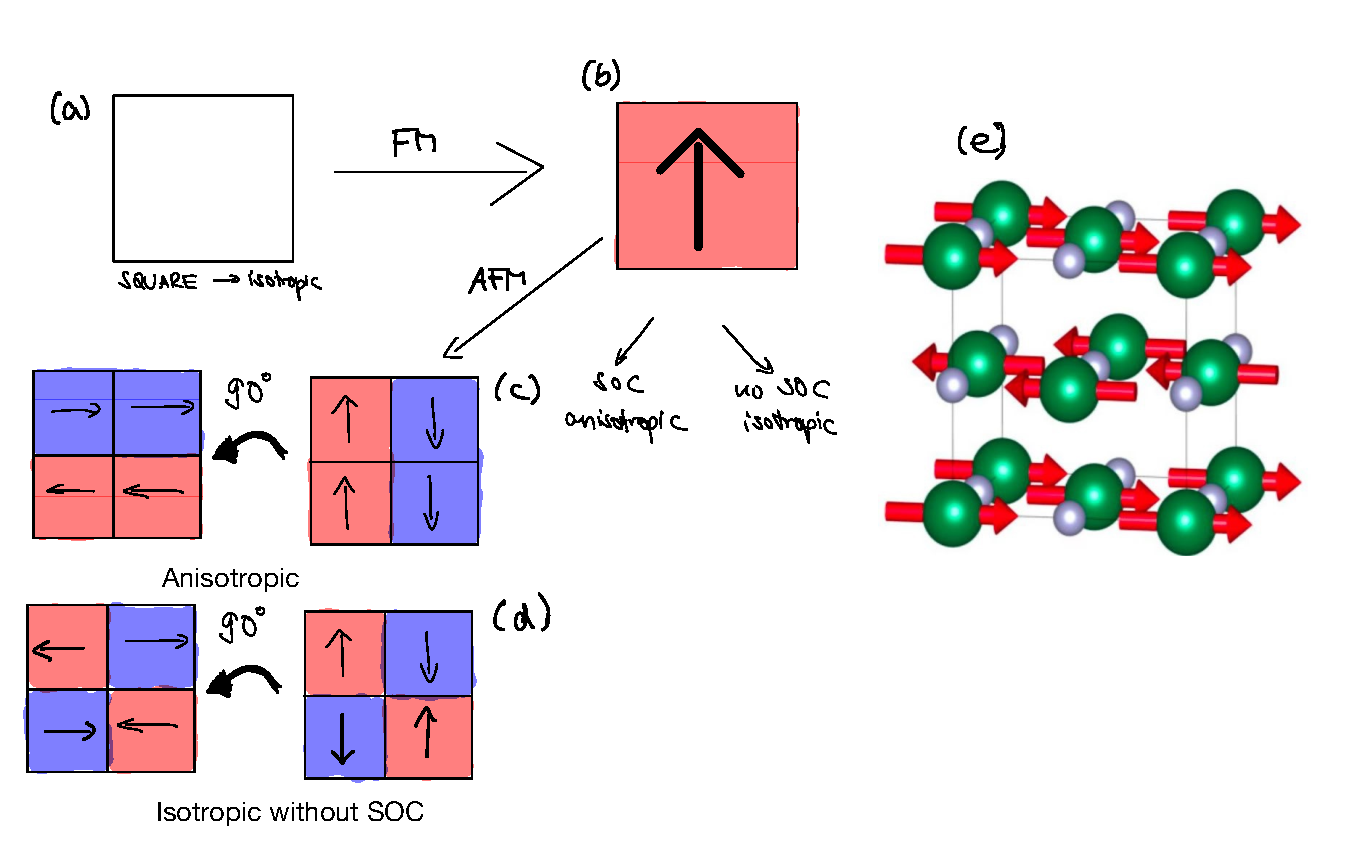
\includegraphics[width=1\linewidth]{img/MnN_sketch_v2}
	\caption{(a) A square lattice without magnetic order exhibits isotropic conductivity $\sigma_{xx} = \sigma_{yy}$. (b) A FM magnetic order allows for AMR $\sigma_{xx} \neq \sigma_{yy}$ only in presence of SOC. (c,d) Including multiple MSL {\color{blue} (red and blue) allows for AMR in a collinear AFM even in absence of SOC if the $90^\circ$ real-space rotation symmetry is broken by the magnetic order: (c) Symmetry-breaking due to the rotation of the FM planes. (d) The FM planes remain invariant under real-space rotation. The conductivity will remain isotropic due to the linearity of the conductivity tensor.} (e) Crystalline structure with magnetic order of MnN, reproduced from Ref.~\cite{Dunz:2020}. The magnetic order breaks the $90^\circ$ real-space rotation symmetry and allows for non-relativistic AMR.}
	\label{fig:mnnsketch}
\end{figure}

Since magnetic order is a spontaneous effect, realizing AMR due to the measurement of conductivity along different directions can also make it a spontaneous effect. This is illustrated in Fig.~\ref{fig:mnnsketch}: In a cubic crystal without magnetic order, the conductivity remains isotropic $\sigma_{xx}=\sigma_{yy}=\sigma_{zz}$. A sufficiently simple FM magnetic order ( in a cubic crystal still exhibits isotropic conductivity in absence of SOC, since global spin rotations do not alter the symmetry of the conductivity tensor. If more MSLs are considered, the conductivity can become anisotropic if the magnetic order breaks the $90^\circ$ real-space rotational symmetry (see (Fig.~\ref{fig:mnnsketch}c). This is the case of cubic MnN, which has a rock-salt structure (see ~\ref{fig:mnnsketch}e): Without magnetic order, the conductivity would remain isotropic. However, the cation (manganese) magnetic moments, prefer an A-type AFM order and in choosing
the direction of the ferromagnetic planes (e.g. $xy$-planes),
anisotropy arises (in that case, $\sigma_{zz}$ is different from
$\sigma_{xx}=\sigma_{yy}$)~\cite{Granville:2005}. This effect in itself is non-relativistic in nature, since the magnetic order breaks crystalline symmetries even without SOC, which creates AMR. \\

Calculations based on density functional theory (DFT as detailed in Appendix A, $a=b=c$), show that $\hbar\omega^p_{xx}=5.87$~eV and $\hbar\omega^p_{zz}=5.23$~eV so that, assuming isotropic scattering, $\sigma_{xx}/\sigma_{zz}-1\approx 26$~\% according to~ Eq. \ref{eq_Boltzmann_2}.

Magnetic order leads to a distortion of lattice but this effect has only minor influence on such transport anisotropy --- for example, $a/c=0.4256/0.4189$~nm changes $\hbar\omega^p_{xx}$ to $5.88$~eV and $\hbar\omega^p_{zz}$ to 5.10~eV.

\subsection{Intrinsic AMR due to Manipulation of the Magnetic Order}
\label{sec_I_Kagome}

\begin{figure}[h!]
	\centering
	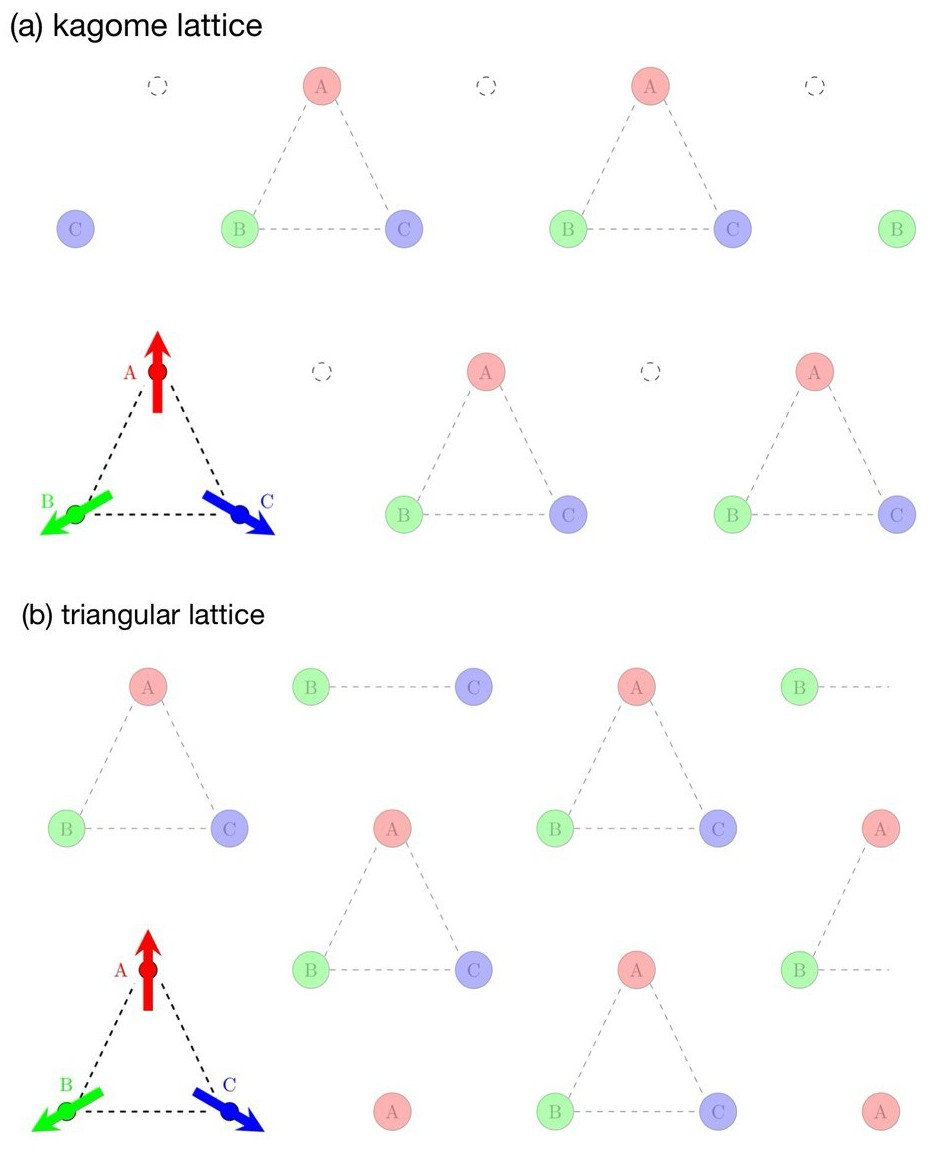
\includegraphics[width=1\linewidth]{img/kagome_triangular_11.jpg}
	\caption{Schematic image of (a) the kagome lattice and (b) the triangular lattice with non-collinear magnetic order. The three magnetic moments in the magnetic unit cell are shown in red (A), green (B) and blue (C). The net magnetic moment is zero. While the magnetic unit cell of both configurations is th same, the regular vacancy of the kagome lattice (dashed circle) distinguishes the two. In practice, the vacancy can be filled with a non-magnetic atom.}
	\label{fig:kagome_triangular}
\end{figure}

\begin{figure}[h!]
	\centering
	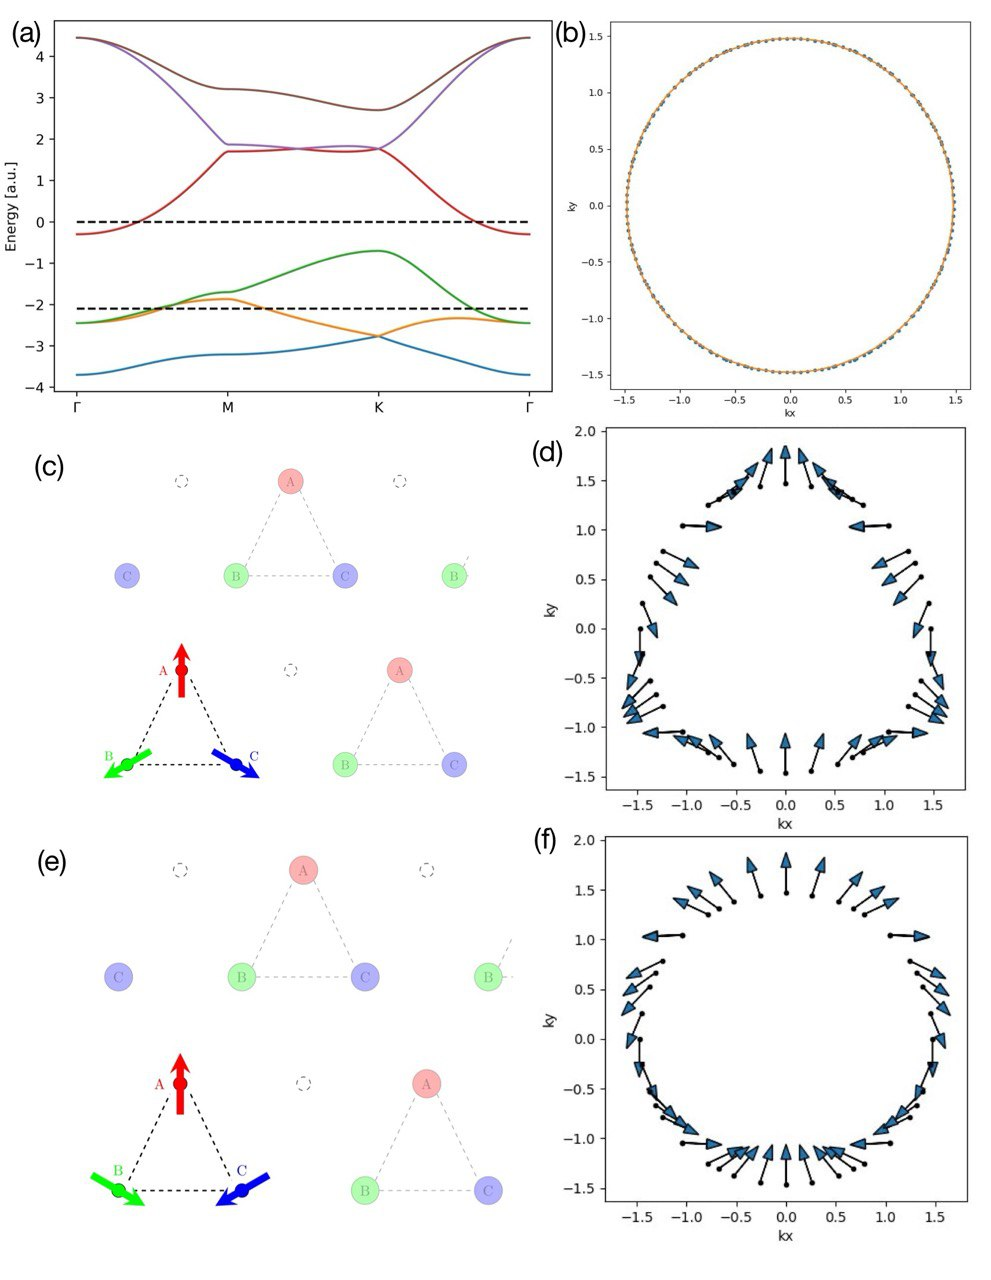
\includegraphics[width=1\linewidth]{img/overview_Kagome_phase1a}
	\caption{Results for two compensated magnetic configuration on the kagome lattice. (a) The band structure is spin-split. Permutation, which corresponds to a $180^\circ$ global spin rotation around the \textit{y}-axis, does not change the band structure. (b) The Fermi surface at $E_F = 0$ (as indicated by the dashed line in (a)) is represented by the blue dots. The orange circle is shown for illustration. Since the FS and the circle overlap, this system has an isotropic FS and does not show intrinsic AMR. (c), (e) The magnetic unit cells of two compensated magnetic configurations and (d), (f) their respective k-space spin texture at the same Fermi level. While the band structure and Fermi surface is unaffected by permutation within the magnetic unit cell, the spin texture changes. The spin texture is entirely in the \textit{xy}-plane. The $\hat{z}$-component (not shown) of the spin texture is zero.}
	\label{fig:totalkagomephase1a}
\end{figure}


{\color{blue} Contrary to MnN, where the magnetic order itself breaks the real-space rotational symmetry, non-collinear magnetic order on a kagome and triangular lattice conserves the symmetry of the conductivity tensor. In this section, we study how intrinsic AMR can be induced by manipulating the magnetic order. The type of magnetic order we consider is a} non-collinear (no SSA), coplanar ($m_{z,i} = 0, \forall i$) and fully compensated ($\sum_i \vec{m}_i = 0$) magnetic order as indicated in Fig.~\ref{fig:kagome_triangular}, as such magnetic order can be found in many materials~\cite{Siddiqui:2020}. This can be realized by considering a simple next-neighbor (NN) Heisenberg exchange term $\sum_{<ij>} -J_{ij} \vec{S}_i \vec{S}_j$ with $J_{ij} = -1$. On a kagome and a triangular lattice, the non-collinear magnetic order will form to avoid frustration. As mentioned before, global spin rotations do not alter the symmetry of the conductivity tensor. This is illustrated in Fig.~\ref{fig:totalkagomephase1a} (d) and (f): While the band structure (BS) and Fermi surface (FS) remain unchanged, the spin texture is rotated by $180^\circ$ around the \textit{y}-axis. This is, because the two corresponding magnetic configurations (see Fig.~\ref{fig:totalkagomephase1a}(c) and (e)) are permutation of each other, which corresponds to a global spin rotation of $180^\circ$ around the \textit{y}-axis. Hence, intrinsic AMR cannot be found. 


\begin{figure}
	\centering
	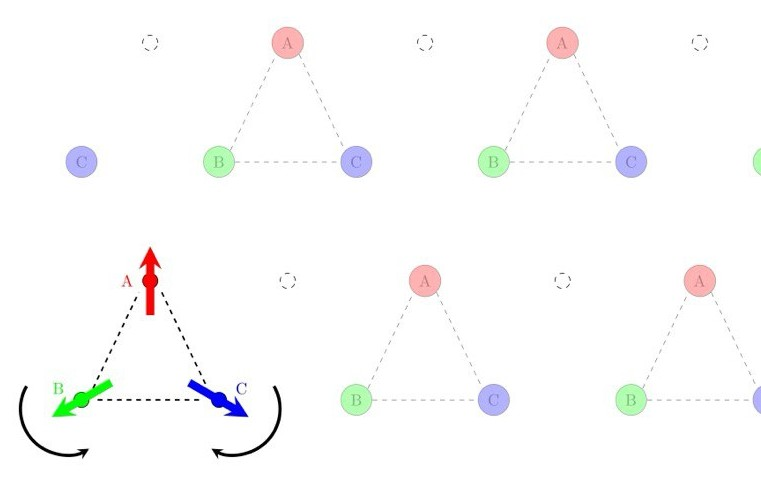
\includegraphics[width=0.9\linewidth]{img/kagome_rotation}
	\caption{Illustration of the rotation of the moments B (counterclockwise) and C (clockwise) by the same angle $\alpha$}
	\label{fig:kagomerotation}
\end{figure}


Next, we are individually rotating the magnetic moments
within the $xy$-plane as shown in Fig.~\ref{fig:kagomerotation}: While moment $A$ remains fix, moment $B$ is rotated counterclockwise and moment $C$ is rotated clockwise, illustrating the effect of a magnetic field in the negative $-\hat{y}$-direction. Moments $B$ and $C$ are rotated by the same angle $\alpha$. Using this notion, we would like to draw the attention to a few special cases: $\alpha = 0^\circ (120^\circ)$ corresponds to the compensated states shown in Fig.~\ref{fig:totalkagomephase1a} (c) (Fig.~\ref{fig:totalkagomephase1a} (e)), $\alpha = 240^\circ$ corresponds to the ferromagnetic states with magnetization along $+\hat{y}$ and $\alpha = 60^\circ$ corresponds to a collinear ferrimagnetic state. For all $\alpha \neq 0^\circ, 120^\circ, 240^\circ$ a partially compensated in-plane magnetization (PCM) exists. 

We found an anisotropic FS (see Fig.~\ref{fig:asymmFS} for the example of $\alpha = 24^\circ$ and $36^\circ$) and thus, intrinsic AMR for all PCM cases. The isotropic cases are the fully compensated ($\alpha = 0^\circ$) and the FM case. Applying the \textit{Symmetr} code~\cite{Symmetr} to get the generators of the real-space symmetries, we find that the WF cases break both a $60^\circ$ and $120^\circ$ rotational symmetries in the \textit{xy}-plane, while the fully compensated and the FM case, conserve at least one of them. 
Different to our previous anticipation~\cite{Ritzinger:2023}, the anisotropy in the collinear ferrimagnetic case ($\alpha = 60^\circ$) indicates that the non-collinear magnetic order is not needed to generate the effect, if the real-space symmetry is low enough as already shown in MnN in the previous section. The AMR in the PCM cases is not due to existence of a net moment, but because of symmetry breaking, which could even exist in absence of a net moment. Similarily, in MnTe, despite the existence of a \textit{weak ferromagneticlike signal} (WFL), the AHE was not attributed to the latter, however the AHE is due to an imbalance of magnetic domains with Hall contributions that cancel out. This imbalance causes the WFL and thus the WFL serves as measure of this imbalance~\cite{Kluczyk:2024}, similar to the magnetization in the PCM cases serves as measure of the symmetry breaking.

\begin{figure}
	\centering
	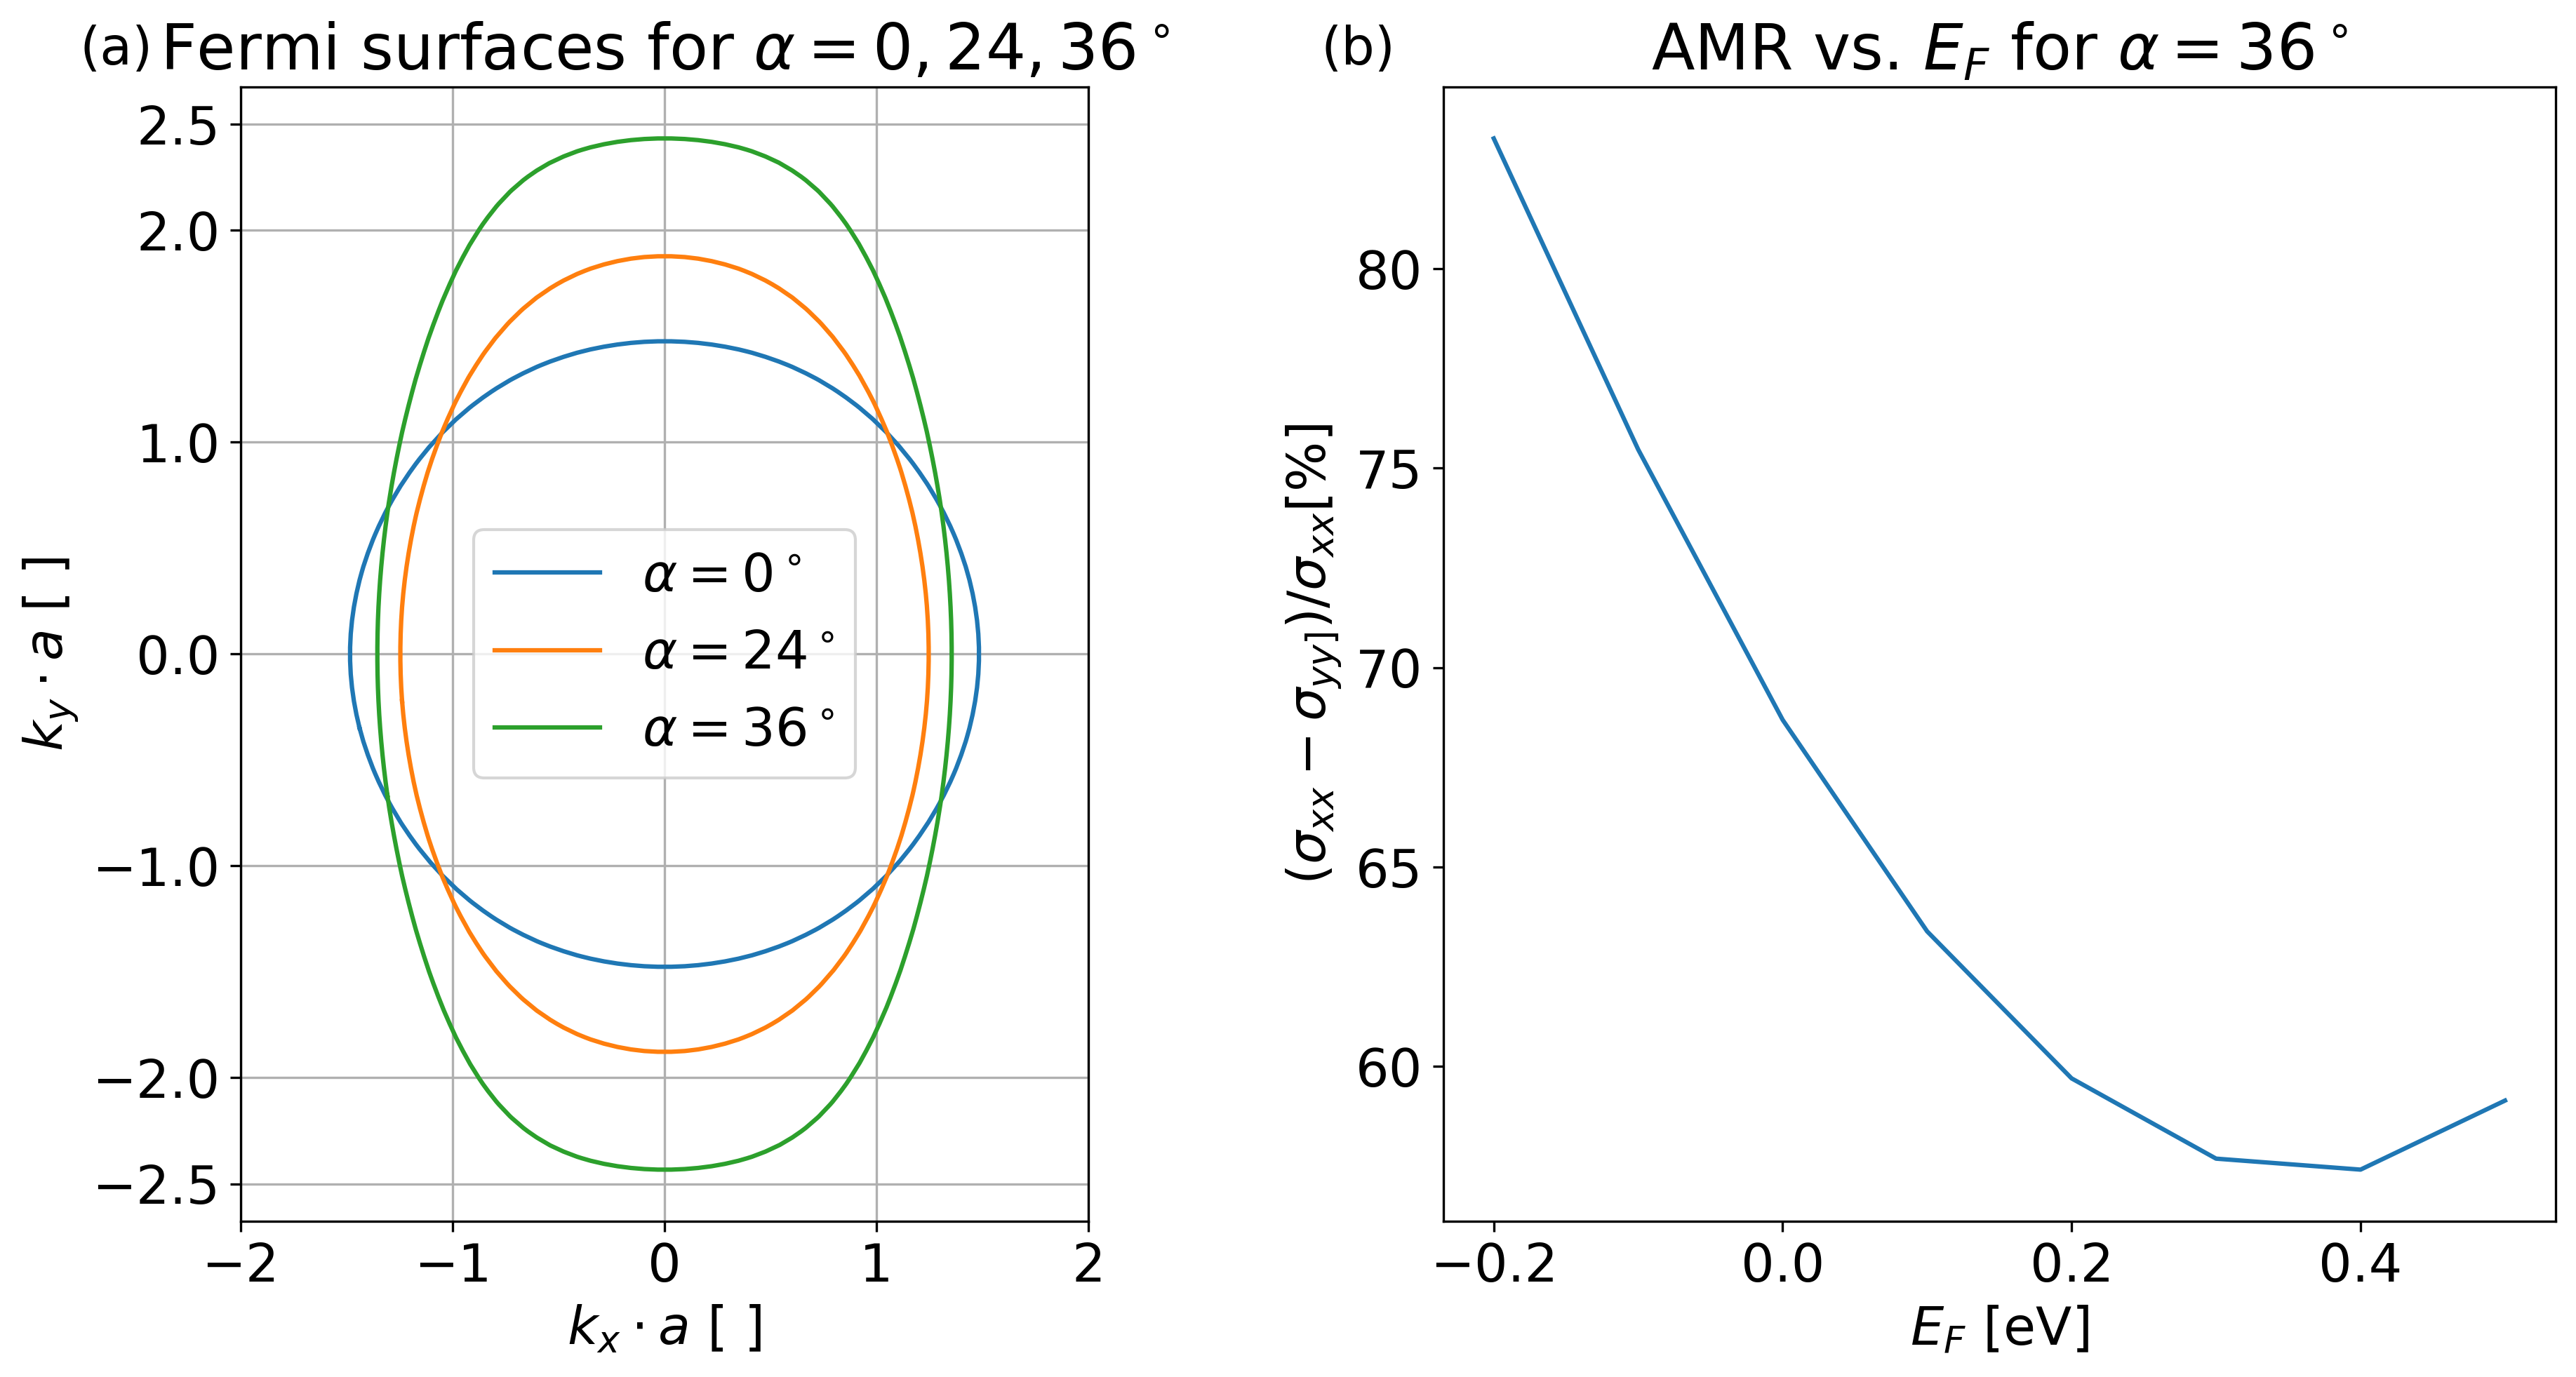
\includegraphics[width=\linewidth]{img/fig5}
	\caption{Anisotropy induced by magnetic order. (a) Fermi surface for the magnetic configuration corresponding to a rotation of moments B and C by~$\alpha = 0, 24, 36^\circ$, respectively, as shown in Fig.~\ref{fig:kagomerotation}. $E_F = 0$ ($\alpha = 0, 24^\circ$) and $E_F = 0.1$ ($\alpha = 36^\circ$). For the partially compensated cases $\alpha = 24^\circ$ and $36^\circ$ a pronounced, increasing anisotropy between $\hat{x}$ and $\hat{y}$-directions can be noted. (b) AMR vs. Fermi energy for $\alpha = 36^\circ$. Despite being a qualitative model, limited quantitative statements are possible. Energy scale directly comparable to Fig.~\ref{fig:totalkagomephase1a} (a)}
	\label{fig:asymmFS}
\end{figure}

{\color{red} Discuss Fig.~\ref{fig:fs-rotation} in an appropriate context.} 
Proposing an experiment 'in real material' may be tricky because details of the
magnetic anisotropy can play important role.

\begin{figure}
	\centering
	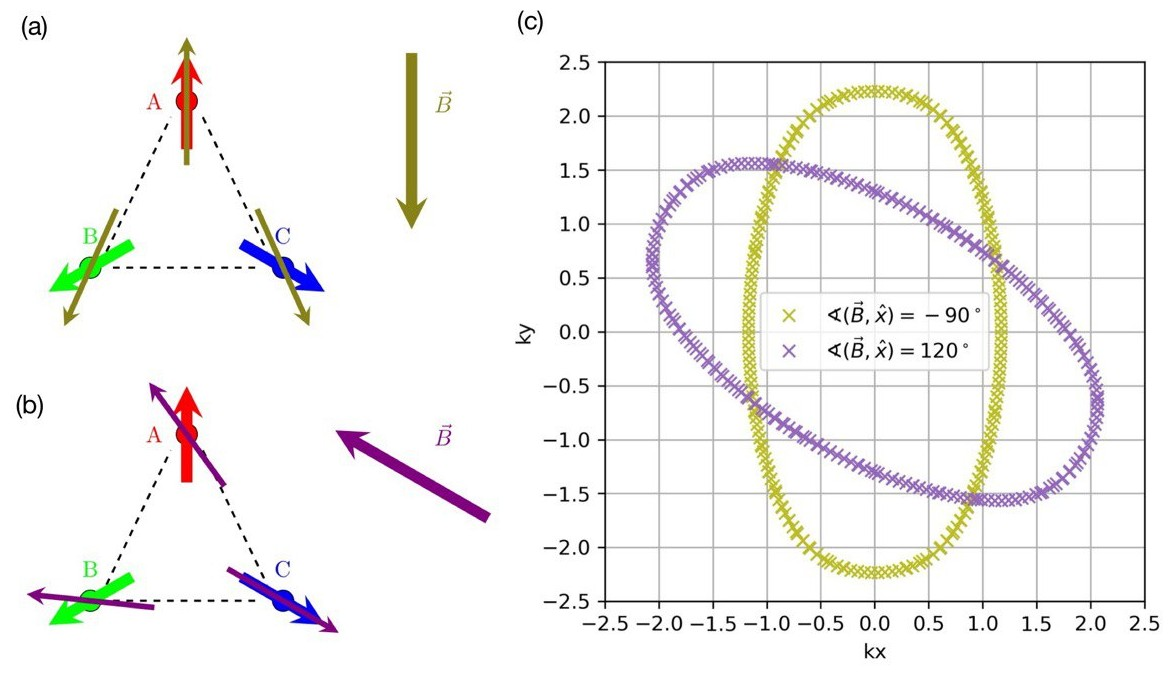
\includegraphics[width=1\linewidth]{img/FS-rotation}
	\caption{Rotation of the warped Fermi surface: 
		%	
		(a) The magnetic field (ochre) was applied in $-\hat{y}$-direction (or $\sphericalangle (\vec{B}, \hat{x}) = -90^\circ$) rotating the moments B and C towards the magnetic field, while leaving A in its original positions. The rotated moments are shown in ochre. (b) Simultaneously, the magnetic field (violet) was applied along $\sphericalangle (\vec{B}, \hat{x}) = 120^\circ$. The rotated moments are shown in violet. (c) The resulting Fermi surfaces (ochre and violet, respectively) are hence rotated by 60$^\circ$, and are not overlapping, resulting in a differing AMR.}
	\label{fig:fs-rotation}
\end{figure}

Now we are turning towards the triangular lattice (see Fig.~\ref{fig:kagome_triangular} (b)). Here, the same operations were applied as for the kagome lattice. In either the fully compensated states, the FM state and the partially compensated PCM cases, no anisotropic FS and thus, no intrinsi AMR was found. Analyzing the real-space symmetries using \textit{Symmetr}~\cite{Symmetr}, we find that all investigated cases are conserving the $60^\circ$ or $120^\circ$ rotational symmetry. 

In summary, we have investigated various magnetic configurations on a kagome and a triangular lattice. The configurations that break the $60^\circ$ and $120^\circ$ real-space rotational symmetry in the \textit{xy}-plane exhibit an anisotropic FS and thus, AMR. These are the non-compensated configurations in the kagome lattice (both non-collinear and collinear ferrimagnetic), yet none of the investigated triangular configuration. This underlines that, while spin and lattice are largely decoupled~\cite{Gonzalez-Hernandez:2024} in absence of SOC, the magnetic order in general does can change the symmetry of the conductivity tensor.


\subsection{A Material Example: Mn$_3$Sn}
\label{sec_I_mat}

{\color{blue} We now apply the insights from the previous subsection to a realistic material: Mn$_3$Sn, a well-studied non-collinear antiferromagnet with a double-layer kagome lattice~\cite{Tomiyashi:1982}. Although known for over six decades~\cite{Cable:1993_a}, Mn$_3$Sn has recently attracted renewed interest due to its large anomalous Hall and Nernst effects, positioning it as a promising material for spintronic applications~\cite{Manna:2018, Chen:2021, Nakatsuji:2015}.
Using structural data from the MAGNDATA database~\cite{Magndata:Mn3Sn} and symmetry analysis via \textit{Symmetr}\cite{Symmetr}, we confirm that the ideal magnetic configuration retains $60^\circ$ and $120^\circ$ real-space rotational symmetries, whereas field-tilted configurations (compare Fig.~\ref{fig:fs-rotation}) break both, consistent with our toy model results.

While our framework assumes field-induced tilts of individual magnetic moments—leading to symmetry-breaking and enabling non-relativistic AMR—this behavior in Mn$_3$Sn is subtle. The strong exchange interactions often cause a rigid rotation of the full spin texture, preserving the $120^\circ$ symmetry~\cite{Tomiyashi:1982, Wu:2023}. However, torque magnetometry has shown that under sufficiently strong magnetic fields, local tilts can occur~\cite{Li:2021}. Additionally, symmetry breaking may also result from anisotropic bond distortions induced by piezomagnetism~\cite{Meng:2024} or hydrostatic pressure~\cite{Singh:2020}, both of which are sensitive to deviations from ideal 3:1 stoichiometry. In off-stoichiometric samples, excess Mn may occupy interstitial or Sn sites~\cite{Gas:2025_a}, potentially contributing to magnetic disorder as suggested in Fig.~\ref{fig:kagome21}. We will examine scattering on such defects in the next section.

In summary, Mn$_3$Sn provides a compelling platform for non-relativistic AMR. When the $60^\circ$ and $120^\circ$ symmetries are broken, anisotropic Fermi surfaces and AMR can emerge—confirming earlier claims by Sharma et al.~\cite{Sharma:2023_a} and in line with our kagome model results.}


\section{Extrinsic AMR}
\label{sec_extrinsic}

{\color{red}  Refer to KV paper again with (Ga,Mn)As ... JZ: FM impurity in FM system is different than FM impurity in AFM system. The change of system is the non-trivial aspect. Careful, depends how I write it }
In this section, we investigate the extrinsic (scattering-dependent) AMR. We will revert to the full treatment of scattering via Eq.~\ref{eq_FermiGoldenRule_1}, assuming magnetic impurities pointing in $\vec{i}$-direction described by the transition matrix matrix $\hat{M} = \hat{S}_i \otimes \hat{1}_{NxN}$, where $\hat{S}_i$ is the $i$-th Pauli spin matrix and $\hat{1}_{NxN}$ is the $N$-dimensional identity matrix, where $N$ is the number of atoms in the unit cell. For simplicity reasons, we will restrict ourselves to impurities either pointing in \textit{x}-direction, as illustrated in Fig.~\ref{fig:kagome21}, which shall be abbreviated as \textit{x}-impurities, and impurities in \textit{y}-direction, denoted as \textit{y}-impurities. It shall be noted that these impurities, which are ferromagnetically aligned in a single direction, introduce a symmetry breaking to the system. This might seem counterintuitive at first, since impurities in a real material would likely be nearly statistically equal distributed among all directions of space. {\color{red} We justify} this ferromagnetic alignment by assuming that the magnetic impurities are only weakly coupled to the crystal and can be aligned by a external magnetic field, which is not sufficient to overcome the exchange interaction and thus, to manipulate the other magnetic moments.

\begin{figure}
	\centering
	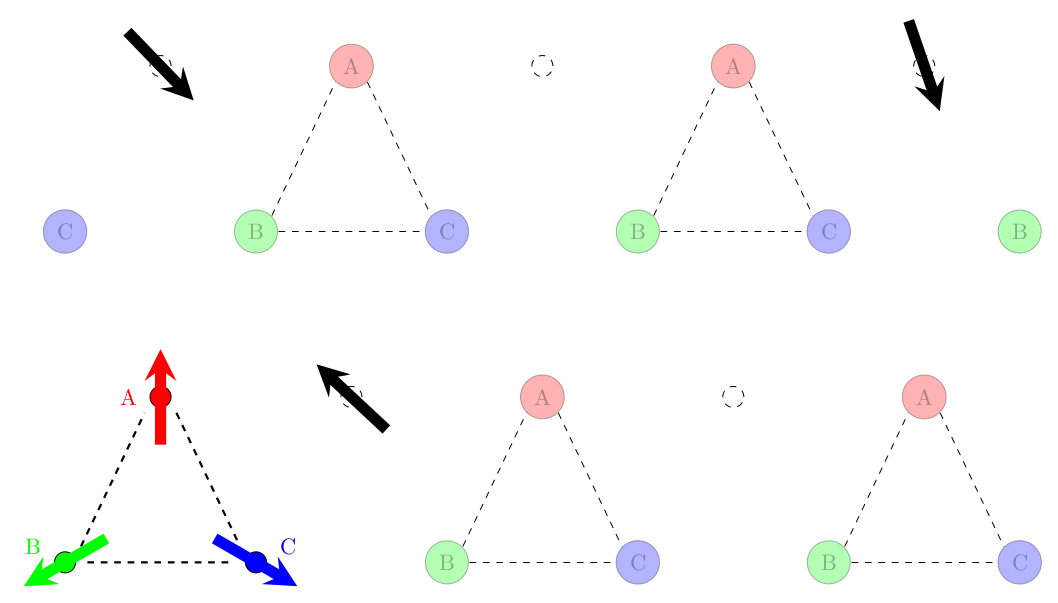
\includegraphics[width=\linewidth]{img/Kagome-impurity_v2}
	\caption{Illustration of unaligned magnetic impurities (black) in the matrix of a kagome lattice. In Mn$_{3+x}$Sn$_{1-x}$ (where only a fraction of $x$ Sn atoms is replaced by additional Mn) this could correspond to substitutional impurities. {\color{blue} The black arrows serve illustrative purposes as the concentration of impurities would be much lower.}
	}
	\label{fig:kagome21}
\end{figure}


As previously in Sec.~\ref{sec_I_Kagome}, we investigate both a kagome and a triangular lattice. We then calculate the conductivities $\sigma_{xx}$ and $\sigma_{yy}$ using the Eqs.~\ref{eq_Boltzmann_1}-\ref{eq_transmatrix}. The results are summarized in table~\ref{T_extrinsic}.\\

\begin{table}
	\begin{tabular}{llll}
		Lattice & Impurity $\hat{M}$ & AMR? & Spin texture \\
		\hline 
		\textbf{Kagome (comp.)} & \textbf{\textit{x}} & \textbf{Yes} & \textbf{\textit{xy}} \\
		\textbf{Kagome (comp.)} & \textbf{\textit{y}} & \textbf{Yes} & \textbf{\textit{xy}} \\
		\textbf{Kagome (PCM)} & \textbf{\textit{x}} & \textbf{Yes} & \textbf{\textit{xy}} \\
		\textbf{Kagome (PCM)} & \textbf{\textit{y}} & \textbf{Yes} & \textbf{\textit{xy}} \\
		\hline 
		Triangular (comp.) & \textit{y} & divergent & \textit{z} \\
		Triangular (PCM) & \textit{y} & No & \textit{zy} \\
	\end{tabular}
	\caption{Results of the extrinsic AMR calculations for kagome and triangular lattice in both compensated and partially compensated magnetic configurations. The impurities as introduced in the text. "Yes" means that AMR was found, hence $\sigma_{xx} \neq \sigma_{yy}$ while for "No" an isotropic behavior was identified, where $\sigma_{xx} = \sigma_{yy}$. The value of the AMR ratio is not stated here, as our model is qualitative. "Divergent" means that both $\sigma_{xx}$ and $\sigma_{yy}$ are divergent or infinite and AMR cannot be defined, originating from a suppressed scattering rate $\Gamma \rightarrow 0$. "Spin texture" indicates the active components of the k-space spin texture at the FS. \textit{xy} indicates that all the spins are within the \textit{xy}-plane and thus $\hat{s}_z = 0$ for all spins. The spin texture serves as a good intuition for whether a certain impurity would lead to suppressed scattering.}
	\label{T_extrinsic}
\end{table}


In the kagome case, for both the \textit{x}- and the \textit{y}-impurity in both the compensated and partially compensated (PCM non-collinear) cases, non-zero extrinsic AMR was found. In the triangular case, no extrinsic AMR has been identified at all. In some cases the results in Tab.~\ref{T_extrinsic} are denoted by \textit{divergent}, which means that both $\sigma_{xx}$ and $\sigma_{yy}$ are divergent or infinite. This originates from a suppressed scattering due to that impurity $\Gamma \rightarrow 0$ and the fact that the inverse scattering rate is part of the Boltzmann equation Eq.~\ref{eq_Boltzmann_1}. Since our model is very simplistic, it is, however, not expected that in a real system the conductivity would diverge.

%%%% moved to App. D
%\begin{figure}
%	\centering
%	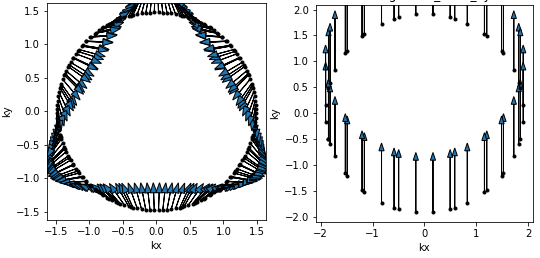
\includegraphics[width=1\linewidth]{img/Combined_Spintexture}
%	\caption{The k-space spin textures of both kagome and triangular lattice for the fully compensated magnetic configurations. (a) In the kagome case, the \textit{z}-component of the spin (not shown) is zero. (b) The spin texture of the triangular case is shown in the $(k_x, k_z)$-plan. All spins point in the \textit{z}-direction. {\color{red}[Apply changes to the figure]}}
%	\label{fig:combinedspintexture}
%\end{figure}

\begin{figure}
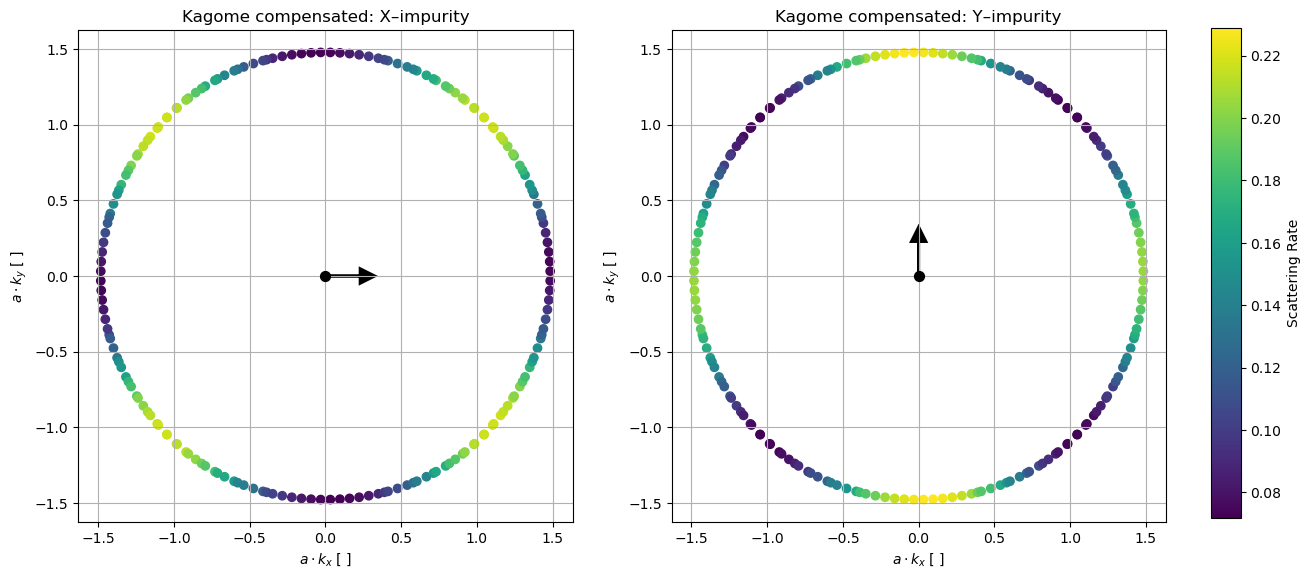
\includegraphics[scale=0.27]{img/fig9.png}
\caption{%New fig. 8 (originally, it was number 9) should contain scatt. rates on FS. Philipp will send it shortly... {\tt :-)}}
Kagome lattice with magnetic impurity. Scattering rate (colour coded) on
the Fermi surface (see dashed line in Fig.~3a) for the same underlying
magnetic order (see Fig.~7) and two orientations of the magnetic impurity.}
\label{fig-09}
\end{figure}

The momentum-space spin textures of the kagome lattice %and the square FM are shown in Fig.~\ref{fig:combinedspintexture}. 
are shown in Fig.~3.  % correct this
Spin textures can be an important tool as already shown in the context of the non-relativistic Edelstein effect~\cite{Gonzalez-Hernandez:2024}.
{\color{red}Well, yes... but PRB 80, 134405~\cite{Trushin:2009_a} is much more relevant here. \textbf{KV paper - formulate}} In our case, it can give us a hint about the possibility of AMR due to its similiarty
{\color{red}(explain please if you really see it :)} The $i$-th component of the spin texture is given by:

\begin{equation}
	S_i (\vec{k}) = \langle \psi_k | \hat{S_i} | \psi_k \rangle
	\label{eq_spintexture}
\end{equation}

where $\psi_k$ is the wave function at $\vec{k}$. The scattering rate $\Gamma$ at the same $\vec{k}$ for a magnetic impurity in direction $i$ described by $\hat{S}_i$:

\begin{equation}	
	{\Gamma_{\vec{k}}} \propto \int_{FS} dk' |\langle \psi_{k'} |\hat{S_i}|\psi_k \rangle|^2
	\label{eq_FermiGoldenRule_2}
\end{equation}

{\color{red} off-diagonal elements on Eq. 10... explain more}\\
where in Eq.~\ref{eq_FermiGoldenRule_2} we ignored $\cos \theta_{vv'}$ and the prefactors, and the delta distribution was evaluated. The integration over $k_z$ does only contribute in a prefactor the system we are looking at is two dimensional. The resulting integral in Eq.~\ref{eq_FermiGoldenRule_2} is a one dimensional integral over the Fermi circle. As can be seen the scattering rate for a magnetic impurity in direction $i$ (Eq.~\ref{eq_FermiGoldenRule_2}) and the $i$-th component of the spin texture are looking very similar, except that the integral over the Fermi surface adds some level of complexity to it. Despite these small differences, it allows us to to explain a part of the results we find in Tab.~\ref{T_extrinsic}. The spin texture of the triangular compensatd pointing in the positive \textit{z}-direction leading to a suppressed scattering for both \textit{x}- and \textit{y}-impurities. In the triangular PCM case, the spin texture acquires some \textit{y}-component as well. Introducing a \textit{y}-impurity will now not lead to a suppressed scattering anymore, yet still not exhbit extrinsic AMR.

In the last part of this section, we investigate at the crystalline AMR, which refers to the anisotropy of conductivity created by the crystalline symmetry. Here, it can be defined as:

\begin{equation}
	AMR^{cry}_{vw} = \frac{\sigma_{ww} (\hat{M} = \hat{S}_w)}{\sigma_{vv} (\hat{M} = \hat{S}_v)}
\end{equation}

where \textit{v} and \textit{w} are two arbitrary directions (e.g. \textit{x} and \textit{y}). The crystalline AMR is thus defind as the quotient as the longitudinal conductivity in \textit{v}-direction for a magnetic impurity in the same direction with the longitudinal conductivity in \textit{w}-direction for a magnetic impurity in the same direction. In both numerator and denominator are thus longitudinal conductivities with parallel aligned impurity. The resulting anisotropy $AMR^{cry}_{vw} \neq 1$ would thus arise only from the influence of the crystal directions. Calculating the respective quantities for the kagome lattice, we indeed find non-zero crystalline AMR.


\section{Summary and Conclusions}
\label{sec_Sum}

In this paper, we have investigated several pathways to realize an anisotropy of conductivity due to magnetic order in the absence of SOC, thus non-relativistic AMR: The magnetic order must break the real-space rotational symmetry of the crystal. In the case of cubic MnN, the A-type AFM order breaks the $90^\circ$ rotational symmetry, exhibiting AMR as a spontaneous effect. In a kagome lattice, the $60^\circ$ and $120^\circ$ rotational symmetries need to be broken, which can be achieved by manipulating the magnetic moments due to an external field. We have suggested an experimental setup to confirm these findings. We have applied those findings to the well-studied non-collinear AFM and spintronic application candidate Mn$_3$Sn, confirming that the $60^\circ$ and $120^\circ$ rotational symmetries need to be broken to exhibit AMR. We have discussed that a field-dependent metal-insulator-transition is an extreme version of that effect, as shown in antiferromagnetic EuTe$_2$. In this paper's second part, we investigated extrinsic AMR depending on ordered magnetic impurities. We found that a suitable impurity can induce AMR in the previously isotropic fully compensated magnetic configuration on a kagome lattice.

Our study calls for further investigations: The model considerations can be extended to include more MSLs as the lattice per se does not predetermine the number of MSLs~\cite{Hayami:2020, Rusnacko:2019}.

A database of materials exhibiting non-relativistic AMR determined by the principles laid out in this paper is desirable. Good candidates are materials with a more complex magnetic order, such as RbFe(MoO$_4$)$_2$ or, e.g., skyrmion host materials. Furthermore, a word of caution: Our model is highly simplistic as it only contains a hopping term and a Heisenberg exchange term. More realistic and complex contributions, such as different atomic orbitals, the crystal field, or the contributions of phonons and magnons, are missing to date, as well as any many-body interactions and correlations. In the exchange, more complicated (often mid-range) pairings of moments are ignored, as well as higher-order contributions such as the Dzyaloshinsky-Moriya interaction, which can play a role in such non-collinear systems. It has to be reminded that the spin moments are not just dipole arrows pointing in a direction, but they are spin densities, which also contain higher multipoles.


\section*{Acknowledgments}

Our work benefited from discussions with folks interested in AMR...
we express our gratitude to them as well as to funding sources from GA\v{C}R (under contract 22-21974S).
 
\begin{appendix}

\section{Ab initio calculations}
\label{apx_A}

$\hbar\omega^p_{xx}=5.87$~eV and $\hbar\omega^p_{zz}=5.23$ for MnN
were obtained using GGA with SOC under assumption of 'perfectly cubic
lattice constants'. When SOC is switched off, the anisotropy of the conductivity remains similar, indicating that the AMR is mainly of non-relativistic nature.

\section{Commentary about the Tight-Binding Model}
\label{apx_B}

From Fig.~\ref{fig:asymmFS} (b), we can see that within our model, limited quantitative statements are possible, at least as long we are keeping within the same lattice and magnetic configurations and keep to a sufficiently small regime. Comparing AMR values quantitatively at vastly different Fermi levels (and thus bands), or the same Fermi levels for different magnetic configuration, or even between different lattices, leads to jumps in the numerical value and does thus not provide ground for a useful analysis. On the contrary, a qualtitative statement is always possible: Given a certain lattice and magnetic configuration, in an isotropic case $\sigma_{xx} / \sigma_{yy} = 1$ for all Fermi energies in all bands, and in an anisotropic case, $\sigma_{xx} / \sigma_{yy} \neq 1$ for all Fermi energies in all bands (although the precise value of $\sigma_{xx} / \sigma_{yy}$ in the anisotropic case is very sensitive to small parameter changes). With changing Fermi level $E_F$, the form of the FS might change as illustrated in Fig.~\ref{fig:kagomenns1phase1adphi0band3ef1}.


\begin{figure}
	\centering
	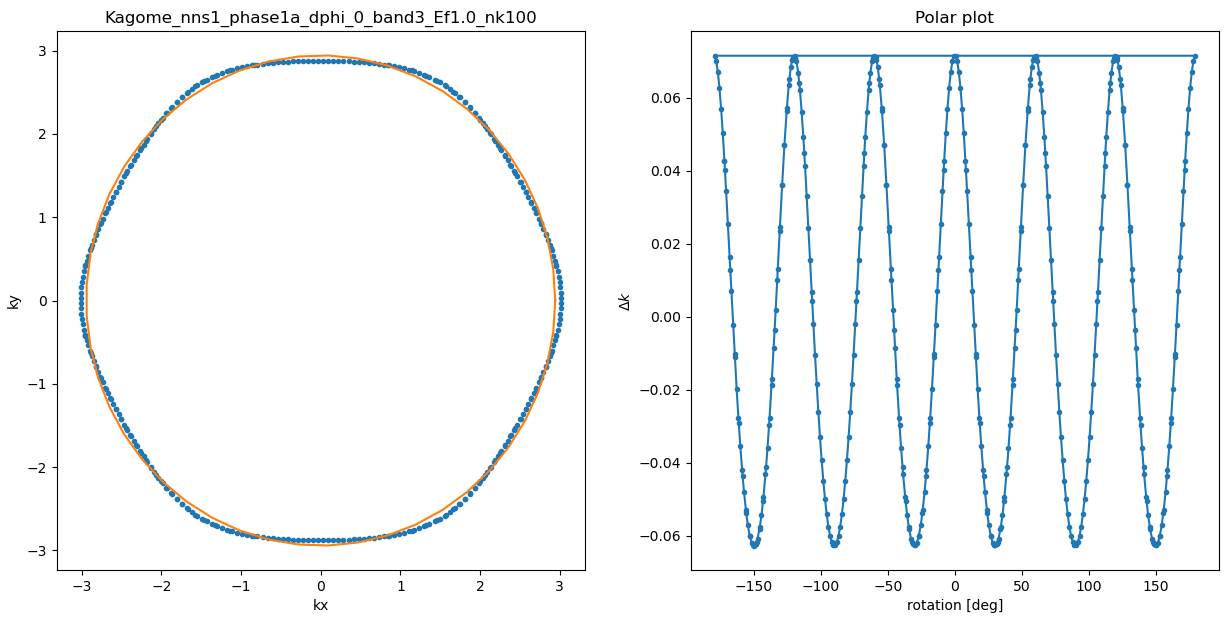
\includegraphics[width=\linewidth]{img/Kagome_nns1_phase1a_dphi_0_band3_Ef1.0_nk100}
	\caption{FS for the fully compensated configuration of the kagome lattice (see Fig.~\ref{fig:totalkagomephase1a} (b)) for a different Fermi level ($E_F = 1$). The FS becomes more hexagonal, which is still isotropic with regards to the conductivity tensor.}
	\label{fig:kagomenns1phase1adphi0band3ef1}
\end{figure}



While in both toy models (see Sec.~\ref{sec_I_Kagome}), we only took next neighbor hopping into account, in the material systems (Mn$_3$Sn, see Sec.~\ref{sec_I_mat}), this did not lead to any realistic results. For Mn$_3$Sn we took 20 next neighbors into account. We chose this number by calculating the Fermi surface and AMR for the material systems using fully ferromagnetic moments as input. Since there is no SOC, the conductivity needs to be isotropic, and any anisotropy can be considered an artifact. We started by next neighbor hopping and increased the number of neighbors until isotropy in the FM state was reached.

\section{An Expanded Phenomenological Model}
\label{apx_phenomodel}

The angle-dependent form of AMR can be expressed phenomenologically in terms of power expansion of the magnetization direction~\cite{Doring:1938,Limmer:2008,DeRanieri:2008} and allows to describe even more complex crystalline AMR signals~\cite{Ritzinger:2021, Gonzalez-Betancourt:2024, NamHai:2012}. However, these models rely on the existence of a SSA as the magnetization or N\'eel vector. In non-collinear systems such SSA does not exist - even in case of weak ferromagnetism induced by an applied magnetic field, it would be likely an oversimplification to ignore the effects of the sublattices. "Local" treatment of effects is not new: For instance, basic AMR models in FMs rely on seperate contributions for spin up and spin down electrons (two-current models)~\cite{Ritzinger:2023}, or the Edelstein effect in non-collinear Mn$_3$Sn can be calculated for each sublattice~\cite{Gonzalez-Hernandez:2024}. Such local approach can be applied to AMR by considering the contributions of each magnetic sublattice (MSL) individually in the phenomenological model, which yields:

\begin{equation}
	\rho_{yy} = \rho_0 + \sum_{m = 1,2,3} \sum_{n = 2, 4, 6, ...} c_{m,n} \cos(n \alpha_m)
	\label{eq_sublattice_AMR}
\end{equation}
where $m$ is the index of the MSL, $n$ is the order of the spherical harmonic, $c_{m,n}$ is the index of the $n$-th harmonic of the $m$-th MSL, and $\alpha_m$ is the angle of the magnetization direction of the $m$-th magnetic moment (assuming an in-plane rotation). The coefficients $c_{m,n}$ can be obtained by fitting where for multiple MSLs measurements for different values of magnetic field $B$ are necessary. The position of the magnetic moments $\alpha_m$ can be obtained from SW models. While this is not going to be a main focus of this work, Eq.~\ref{eq_sublattice_AMR} together with an adequate SW model could help to distinguish the MCA from the AMR.


\section{Dump}

Parts of text and figures moved to here... There was some
inconsistency about Fig.~\ref{fig:combinedspintexture}: is panel (b) from
a triangular or square FM lattice? Fig.~\ref{fig:mn3sn_36deg_FS} supports
the conclusions of Sec.~III.C but it would have to be much improved.

%\subsection{AMR due to Metal-Insulator Transition: EuTe$_2$}
%\label{sec_I_EuTe2}

\begin{figure}
	\centering
	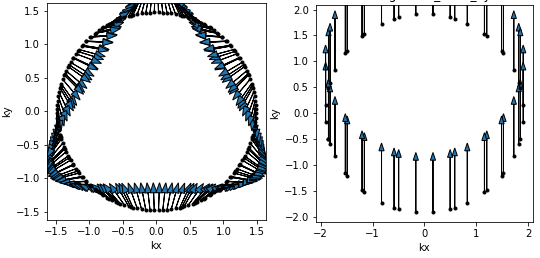
\includegraphics[width=1\linewidth]{img/Combined_Spintexture}
	\caption{The k-space spin textures of both kagome and triangular lattice for the fully compensated magnetic configurations. (a) In the kagome case, the \textit{z}-component of the spin (not shown) is zero. (b) The spin texture of the triangular case is shown in the $(k_x, k_z)$-plan. All spins point in the \textit{z}-direction. {\color{red}[Apply changes to the figure]}}
	\label{fig:combinedspintexture}
\end{figure}

We are now proposing an experiment to show this effect: Applying the magnetic field along a symmetry axis will tilt the magnetic moments, generate a weak ferromagnetic moment (magnetization) and result in AMR due to an anisotropic Fermi surface (see Fig.~\ref{fig:fs-rotation} (a) and (c), ochre). Now, we are rotating the magnetic field by $120^\circ$, so that it points along another symmetry axis. The magnetic moments will tilt in another direction (see Fig.~\ref{fig:fs-rotation} (b)), and result in a rotated FS, which does not overlap with the previous FS (see Fig.~\ref{fig:fs-rotation} (c)), thus leading to another value of AMR. We can now rotate the conductivity measurement from $\sigma_{xx}$ and $\sigma_{yy}$ to $\sigma_{vv}$ and $\sigma_{ww}$, where here $\hat{v} = \hat{x} + 120^\circ$ ($\hat{w} = \hat{y} + 120^\circ$) and recover the original value of the AMR. 

\begin{figure}
        \centering
        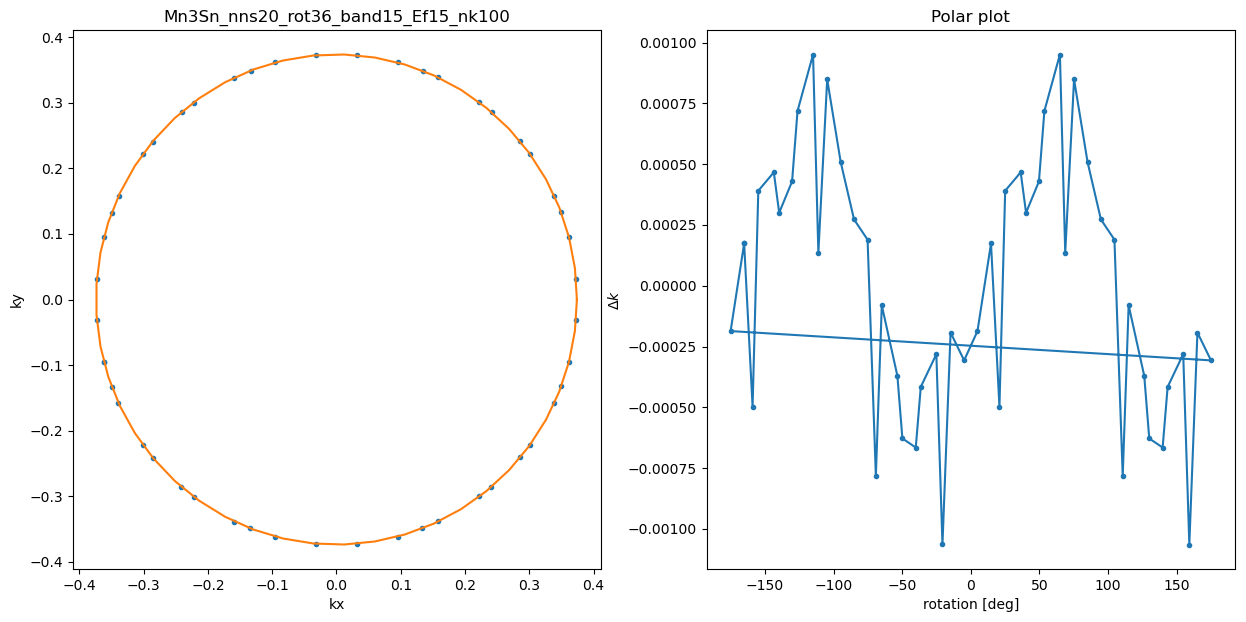
\includegraphics[width=\linewidth]{img/Mn3Sn_nns20_rot36_band15_Ef15_nk100}
        \caption{Non-compensated (WF) case of Mn$_3$Sn. {\color{red} (a) [to be included] Schematics of the tilted magnetic moments}. (b) Simplied FS (blue dots) and, for illustrative reasons, a circle with perfect spherical symmetry (orange) at $E_F = 15$. The shown FS is an intersection through the $k_z = 0$-plane. (c) Deviation of the FS (blue dots in (b)) from the spherical symmetry (orange in (b)): A weak two-fold symmetry is recognizable, which is sufficent to reder the FS sufficiently anisotropic and exhibit AMR}
        \label{fig:mn3sn_36deg_FS}
\end{figure}


\end{appendix}

\def\urlprefix{}
\def\url#1{}\bibliography{lit}
%% %\bibliography{dms-assorted}% 


\begin{thebibliography}{99}

% cut after 20 authors


\bibitem{Thomson:1857} W. Thomson, Proc. R. Soc. Lond. 8, 546 (1857). %(doi:10.1098/rspl.1856.0144)

\bibitem{Ritzinger:2023} P. Ritzinger, K. V\'yborn\'y, R. Soc. Open Sci., 10, 230564 (2023). %DOI: 10.1098/rsos.230564

\bibitem{Alagoz:2015} H. S. Alagoz, J. Desomberg, M. Taheri, F. S. Razavi, K. H. Chow, and J. Jung, Appl. Phys. Lett. 106, 082407 (2015).

\bibitem{Vitayaya:2024} O. Vitayaya, P. Z. Z. Nehan, D. R. Munazat, M. T. E. Manawanbc,  B. Kurniawan, %"Magnetoresistance (MR) properties of magnetic materials", 
RSC Adv. 14, 18617 (2024). %: 10.1039/d4ra01989j


\bibitem{Kriegner:2017} D. Kriegner, H. Reichlova, J. Grenzer, W. Schmidt, E. Ressouche, J. Godinho, T. Wagner, S. Y. Martin, A. B. Shick, V. V. Volobuev, G. Springholz, V. Hol\'{y}, J. Wunderlich, T. Jungwirth, K. V\'{y}born\'{y}, Phys. Rev. B 96, 214418 (2017). %DOI: 10.1103/PhysRevB.96.214418

\bibitem{Gonzalez-Betancourt:2024} R. D. Gonzalez Betancourt, J. Zub\'a\v{c}, K. Geishendorf, P. Ritzinger, B. R\r{u}\v{z}i\v{c}kov\'a, T. Kotte, J. \v{Z}elezn\'y, K. Olejn\'ik, G. Springholz, B. B\"uchner, A. Thomas, K. V\'yborn\'y, T. Jungwirth, H. Reichlov\'a, D. Kriegner, npj Spintronics, 2, 45 (2024). %DOI: 10.1038/s44306-024-00046-z


\bibitem{Volny:2020} J. Voln\'y, D. Wagenknecht, J. \v{Z}elezn\'y, P. Harcuba, E. Duverger–Nedellec, R. H. Colman, J. Kudrnovsk\'y, I. Turek, K. Uhl\'i\v{r}rov\'a, K. V\'yborn\'y, Phys. Rev. Mat. 4, 064403 (2020).% DOI: 10.1103/PhysRevMaterials.4.064403

\bibitem{Zubac:2021} J. Zub\'a\v{c}, Z. Ka\v{s}par, F. Krizek, F\"orster, R. P. Campion, V. Nov\'ak, T. Jungwirth, K. Olejn\'ik, Phys. Rev. B 104, 184424 (2021). %DOI: 10.1103/PhysRevB.104.184424

\bibitem{Wadley:2016} P. Wadley, B. Howells, J. \v{Z}elezn\'y, C. Andrews, V. Hills, R. P. Campion, V. Nov\'ak, K. Olejn\'ik, F. Maccherozzi, S. S. Dhesi, S. Y. Martin, T. Wagner, J. Wunderlich, F. Freimuth, Y. Mokrousov, J. Kune\v{s}, J. S. Chauhan, M. J. Grzybowski, A. W. Rushforth, K. W. Edmonds, B. L. Gallagher, T. Jungwirth, Science 351, 6273 (2016). %DOI: 10.1126/science.aab1031

\bibitem{Kabara:2017} K. Kabara, M. Tsunoda, S. Kokado, AIP Adv. 7, 056416 (2017). %DOI:10.1063/1.4974065

\bibitem{Bakonyi:2022} I. Bakonyi, F. D. Czeschka, L. F. Kiss, V. A. Isnaini, A. T. Krupp, K. Palot\'as, S. Zsurzsa, L. P\'eter, arXiv:2203.11568 [cond-mat.mtrl-sci] (2022). %DOI: 10.48550/arXiv.2203.11568.

\bibitem{Gonzalez-Hernandez:2024} R. Gonz\'alez-Hern\'andez, P. Ritzinger, K. V\'yborn\'y, J. \v{Z}elezn\'y, A. Manchon, Nat. Commun., 15, 7663 (2024).% DOI: 10.1038/s41467-024-51565-6

\bibitem{Nadvordnik:2021} L. N\'{a}dvorn\'{i}k, M. Borchert, L. Brandt, R. Schlitz, K. A. de Mare, K. V\'{y}born\'{y}, I. Mertig, G. Jakob, M. {Kl\"{a}ui}, S. T.B. Goennenwein, M. Wolf, G. Woltersdorf, T. Kampfrath, Phys. Rev. X 11, 021030 (2021). %DOI: 10.1103/PhysRevX.11.021030

\bibitem{Park:2021} J.‑H. Park, H.‑W. Ko, J.‑M. Kim, J. Park, S.‑Y. Park, Y. Jo, B.‑G. Park, S. K. Kim, K.‑J. Lee, K.‑J. Kim, Sci. Rep. 11, 20884 (2021).% DOI: 10.1038/s41598-021-00374-8

\bibitem{Kato:2008} T. Kato, Y. Ishikawa, H. Itoh, J.-i. Inoue, Phys. Rev. B 77, 233404 (2008). %DOI: 10.1103/Phys-RevB.77.233404

\bibitem{Velev:2005} J. Velev, R. F. Sabirianov, S. S. Jaswal, E. Y. Tsymbal, Phys. Rev. Lett. 94, 127203 (2005). %DOI: 10.1103/PhysRevLett.94.127203

\bibitem{Zeng:2020} F. L. Zeng, Z. Y. Ren, Y. Li, J. Y. Zeng, M. W. Jia, J. Miao, A. Hoffmann, W.Zhang, Y. Z. Wu, Z. Yuan, Phys.Rev. Lett. 125, 097201 (2020). %DOI: 10.1103/PhysRevLett.125.097201

\bibitem{Kato:2007} T. Kato, Y. Ishikawa, H. Itoh, J. Inoue, phys. stat. sol. (b) vol. 244, 12, 4403 - 4406 (2007). %DOI:10.1002/pssb.200777260

\bibitem{Zhang:2017} Y. Zhang, Y. Sun, H. Yang, J. \v{Z}elezn\'y, S. P. P. Parkin, C. Felser, B. Yan, Phys. Rev. B 95, 075128 (2017). %DOI: 10.1103/PhysRevB.95.075128

\bibitem{Nagaosa:2010} N. Nagaosa, J. Sinova, S. Onoda, A. H. MacDonald, N. P. Ong, Rev. Mod. Phys. 82, 1539 (2010). %DOI: 10.1103/RevModPhys.82.1539

\bibitem{Dong:2025_a} M. Q. Dong, Z. X. Song, Z.-X. Guo,
Phys. Rev. B 111, 174447 (2025).

\bibitem{Doring:1938} W. D\"oring, Ann. Phys. 424, 259-276
(1938). %DOI: 10.1002/andp.19384240306
  
\bibitem{Ritzinger:2021} P. Ritzinger, H. Reichlov\'a, D. Kriegner, A. Markou, R. Schlitz, M. Lammel, D. Scheffler, G. H. Park, A. Thomas, P. St\v{r}eda, C. Felser, S. T. B. Goennenwein, K. V\'yborn\'y, Phys. Rev. B, 104, 094406 (2021)

\bibitem{Sato:2019} T. Sato, S. Kokado, M. Tsujikawa, T. Ogawa, S. Kosaka, M. Shirai, M. Tsunoda, Appl. Phys. Express 12, 103005 (2019)

\bibitem{DeRanieri:2008} E. De Ranieri, A. W. Rushforth, K. V\'yborn\'y, U. Rana, E. Ahmad, R. P. Campion, C, T, Foxon, B. L. Gallagher, A. C. Irvine, J. Wunderlich, New J. Phys. 10, 065003 (2008).% DOI: 10.1088/1367-2630/10/6/065003


\bibitem{NamHai:2012} P. Nam Hai, D. Sasaki, L. Duc Anh, M. Tanaka, Appl. Phys. Lett. 100, 262409 (2012). %DOI:10.1063/1.4730955

\bibitem{Dong:2023} M. Q. Dong, Z.-X. Guo , X. R. Wang, Phys. Rev. B 108, L020401 (2023). % DOI: 10.1103/PhysRevB.108.L020401

\bibitem{Bonbien:2022} V. Bonbien, F. Zhuo, A. Salimath, O. Ly, A. Abbout, A. Manchon, J. Phys. D: Appl. Phys. 55, 103002 (2022)

\bibitem{Zhou:2020} X. F. Zhou, X. Z. Chen, Y. F. You, L. Y. Liao, H. Bai, R. Q. Zhang, Y. J. Zhou, H. Q. Wu, C. Song, F. Pan, Phys. Rev. Appl. 14, 054037 (2020). %DOI: 10.1103/PhysRevApplied.14.054037


\bibitem{Manna:2018} K. Manna, Y. Sun, L. Muechler, J. K\"uebler, C. Felser, %"Heusler, Weyl and Berry", 
Nat. Rev. Mater. 3, 244-256 (2018). %DOI: 10.1038/s41578-018-0036-5

\bibitem{Jungwirth:2024} T. Jungwirth, R. M. Fernandes, E. Fradkin, A. H. MacDonald, J. Sinova, L. \v{S}mejkal, arXiv:2411.00717v2 [cond-mat.mtrl-sci] (2025) 

\bibitem{BirkHellens:2023} A. Birk Hellenes, T. Jungwirth, R. Jaeschke-Ubiergo, A. Chakraborty, J. Sinova, L. \v{S}mejkal, arXiv:2309.01607v3 [cond-mat.mes-hall]

\bibitem{Yang:2021} H. Yang, Q. Liu, Z. Liao, L. Si, P. Jiang, X. Liu, Y. Guo, J. Yin, M. Wang, Z. Sheng, Y. Zhao, Z. Wang, Z. Zhong, R.-W. Li, Phys. Rev. B 104, 214419 (2021).
%(doi:10.1103/PhysRevB.104.214419)

\bibitem{Vyborny:2009} K. V\'{y}born\'{y}, J. Ku\v{c}era, J. Sinova, A. W. Rushforth, B. L. Gallagher, T. Jungwirth, Phys. Rev. B 80, 165204 (2009)%. DOI: 10.1103/PhysRevB.80.165204

\bibitem{Vyborny:2009_a} K. V\'yborn\'y, A. A. Kovalev, J. Sinova, T. Jungwirth, Phys. Rev. B 79, 045427 (2009). % DOI: 10.1103/PhysRevB.79.045427

\bibitem{Symmetr} J. \v{Z}elezn\'y, Linear response symmetry. Bitbucket \url{https://bitbucket.org/zeleznyj/linear-response-symmetry} (2024)

\bibitem{Dunz:2020} M. Dunz, T. Matalla-Wagner, M. Meinert, Phys. Rev. Research 2, 013347 (2020) %DOI: 10.1103/PhysRevResearch.2.013347

\bibitem{Granville:2005} S. Granville, B. J. Ruck, F. Budde, A. Koo, J. E. Downes, H. J. Trodahl, A. Bittar, N. Strickland, G. V. M. Williams, W. R. L. Lambrecht, T. Learmonth, Kevin E. Smith, V. J. Kennedy, A. Markwitz, T. Schmitt, Phys. Rev. B 72, 205127 (2005). % DOI: 10.1103/PhysRevB.72.205127

\bibitem{Siddiqui:2020} S. A. Siddiqui, J. Sklenar, K. Kang, M. J. Gilbert, A. Schleife, N. Mason, A. Hoffmann, J. Appl. Phys. 128, 040904 (2020). %doi.org/10.1063/5.0009445

\bibitem{Kluczyk:2024} K. P. Kluczyk, K. Gas, M. J. Grzybowski, P. Skupi\'nski, M. A. Borysiewicz, T. Fas, J. Suffczy\'nski, J. Z. Domagala , K. Grasza, A. Mycielski, M. Baj , K. H. Ahn , K. V\'yborn\'y, M. Sawicki, M. Gryglas-Borysiewicz, Phys. Rev. B 110, 155201 (2024)

\bibitem{Cable:1993_a} J. W. Cable, N. Wakabayasi, P. Radhakrishna, Phys. Rev. B 48, 6159 (1993). %DOI: 10.1103/PhysRevB.48.6159

\bibitem{Chen:2021} T. Chen, T. Tomita, S. Minami, M. Fu, T. Koretsune, M. Kitatani, I. Muhammad, D. Nishio-Hamane, R. Ishii, F. Ishii, R. Arita, S. Nakatsuji, Nat. Commun. 12, 572 (2021). %DOI: 10.1038/s41467-020-20838-1; 

\bibitem{Nakatsuji:2015} S. Nakatsuji, N. Kiyohara, T. Higo, \textit{Nature} 527, 212–215 (2015). %DOI: 10.1038/nature15723


\bibitem{Gas:2025_a} K. Gas, J.-Y. Yoon, Y. Sato, H. Kubota, P. D\l{l}u\.{z}ewski, S. Kret, J. Z. Domagala, Y. K. Edathumkandy, Y. Takeuchi, S. Kanai, H. Ohno, M. Sawicki, S. Fukami, APL Mater. 13, 041105 (2025). %10.1063/5.0254918


\bibitem{Tomiyashi:1982} S. Tomiyoshi, Y. Yamaguchi, J. Phys. Soc. Jap. 51, 2478 (1982)

\bibitem{Magndata:Mn3Sn}
\texttt{https://www.cryst.ehu.es/magndata/index.php?index=0.199}, 2024-08-23, 12:01

\bibitem{Wu:2023} M. Wu, K. Kondou, T. Chen, S. Nakatsuji, Y. Otani, AIP Adv. 13, 045102 (2023). %DOI: 10.1063/5.0138208

\bibitem{Singh:2020} C. Singh, V. Singh, G. Pradhan, V. Srihari, H. K. Poswal, R. Nath, A. K. Nandy, A. K. Nayak, Phys. Rev. Research 2, 043366 (2020) % DOI: 10.1103/PhysRevResearch.2.043366

\bibitem{Li:2021} X. Li, S. Jiang, Q. Meng, H. Zuo, Z. Zhu, L. Balents, K. Behnia, arXiv:2109.11122v1 [cond-mat.str-el] (2021)

\bibitem{Meng:2024} Q. Meng, J. Dong, P. Nie, L. Xu, J. Wang, S. Jiang, H. Zuo, J. Zhang, X. Li, Z. Zhu, L. Balents, K. Behnia, Nat. Commun. 15, 6921 (2024)

\bibitem{Sharma:2023_a} V. Sharma, R. Nepal, R. C. Budhani, Phys. Rev. B 108, 144435 (2023). %DOI: 10.1103/PhysRevB.108.144435 

\bibitem{Trushin:2009_a} M. Trushin, K. V\'yborn\'y, P. Moraczewski, A. A. Kovalev, J. Schliemann, T. Jungwirth, Phys. Rev. B 80, 134405 (2009) %DOI: 10.1103/PhysRevB.80.134405

\bibitem{Rusnacko:2019} J. Rusnacko, D. Gotfryd, J. Chaloupka, Phys. Rev. B 99, 064425 (2019)

\bibitem{Hayami:2020} S. Hayami, Y. Yanagi, H. Kusunose, 
%"Spontaneous antisymmetric spin splitting in noncollinear antiferromagnets without spin-orbit coupling". 
Phys. Rev. B 101, 220403(R) (2020). %DOI: 10.1103/PhysRevB.101.220403

\bibitem{Limmer:2008} W. Limmer, J. Daeubler, L. Dreher, M. Glunk, W. Schoch, S. Schwaiger, R. Sauer, Phys. Rev. B 77, 205210 (2008). %DOI: 10.1103/PhysRevB.77.205210 %24 

\bibitem{Brown:1990} P.J. Brown, V. Nunez, F. Tasset, J.B. Forsyth and P. Radhakrishna, Journal of Physics: Condensed Matter 2, 9409-9422 (1990). %10.1088/0953-8984/2/47/015

%\bibitem{Zelezny:2017} J. \v{Z}elezn\'y, Y. Zhang, C. Felser, B. Yan, \textit{Phys. Rev. Lett.} 119, 187204 (2017). %DOI: 10.1103/PhysRevLett.119.187204

%\bibitem{McGuire:1975} T. McGuire, T. Potter. IEEE Trans. Magn. 11, 18 (1975) % (doi:10.1109/TMAG.1975.1058782)

%\bibitem{Ikhlas:2017} M. Ikhlas, T. Tomita, T. Koretsune, M.-T. Suzuki, D. Nishio-Hamane, R. Arita, Y. Otani, S. Nakatsuji, \textit{Nat. Phys.} 13, 1085. %DOI: 10.1038/NPHYS4181

%\bibitem{Park:2018} P. Park, J. Oh, K. Uhl\'i\v{r}ov\'a, J. Jackson, A. De\'ak, L. Szunyogh, K. H. Lee, H. Cho, H.-L. Kim, H. C. Walker, D. Adroja, V. Sechovsk\'y, J.-G. Park, \textit{npj Quantum Materials} 3:63 (2018). %DOI: 10.1038/s41535-018-0137-9.

%\bibitem{Reichlova:2019} H. Reichlova, T. Janda, J. Godinho, A. Markou, D. Kriegner, R. Schlitz, J. Zelezny, Z. Soban, M. Bejarano, H. Schultheiss, P. Nemec, T. Jungwirth, C. Felser, J. Wunderlich,  S.T.B. Goennenwein, \textit{Nat. Commun.} 10:5459 (2019). %DOI: 10.1038/s41467-019-13391-z

%\bibitem{Iwaki:2020} H. Iwaki, M. Kimata, T. Ikebuchi, Y. Kobayashi, K. Oda, Y. Shiota, T. Ono, T. Moriyama,  Appl. Phys. Lett. 116, 022408 (2020). %doi: 10.1063/1.5128241

%\bibitem{Kiyohara:2016} N. Kiyohara, T. Tomita, S. Nakatsuji, Phys. Rev. Appl. 5, 064009 (2016). DOI: 10.1103/PhysRevApplied.5.064009

  
\end{thebibliography}

\end{document}

